% !TEX encoding = UTF-8 Unicode
% !TEX root = ../thesis.tex
% !TEX spellcheck = en-US
%%=========================================



\chapter{Implementation}\label{chap:implementaiton}

% Hololens, UWP, WMR


% and non-functional requirements, which describe  

% \section{Development}
This research project has been in active progression for two semesters and development has effectively been done in two stages. First in October and November 2020 and then from February till May in 2021. During the fall and first stage of development the focus was on the HoloLens 2 and creating a usable act of dissection in augmented reality. The second stage at spring, had a wider scope, with focus on implementing networking, volumetric data and more. During this chapter it will thus be clearly discrete improvements during the first iterations of the product while later iterations will be grouped and focus will be put on specific features or pain points. The final iteration will focus on improvements done from user feedback and the feature set at the end of development.

% A note on the code in 

\section[Iteration 0]{Iteration 0: First steps, importing model}\label{chap:zeroiter}
% 0th iteration: Initializing application, importing and simplifying brain model

\begin{wrapfigure}[12]{r}{0.45\textwidth} 
    \centering
    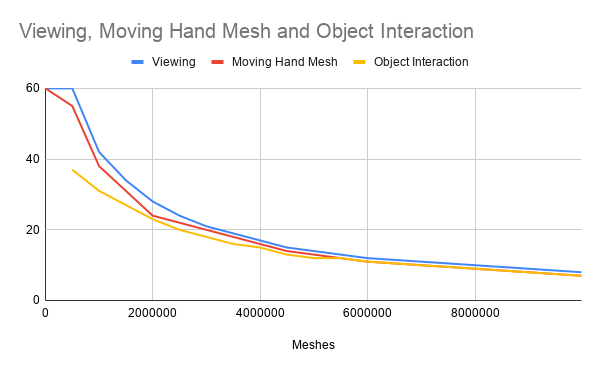
\includegraphics[width=0.45\textwidth]{fig/hololens2polycount}
    \caption{Figure showing frame rate as a function of polygon count on HoloLens 2. Credit: \href{https://community.fologram.com/t/hololens-2-polygon-count-and-frame-rate/49}{Fologram}}
    % \vspace{20pt}
    \label{fig:polycount}
\end{wrapfigure}

The first phase of development started by acquiring the surface model of the WHS rat brain created by \citet{Elden2017}. This was done by simply moving the FBX files from the \nameref{chap:vrvis} application and to a new Unity project. After initializing MRTK by following their \href{https://microsoft.github.io/MixedRealityToolkit-Unity/version/releases/2.2.0/Documentation/GettingStartedWithTheMRTK.html}{Getting Started documentation}, the application was ready to deploy on the HoloLens 2. This resulted in a barely running application as the polygon count of the brain model was orders of magnitude larger than what is recommended to maintain adequate performance on the HoloLens 2, which is in the order of 100,000 polygons shown in \autoref{fig:polycount}. The model used by Elden was scaled to run on workstation computer outputting to an HTC Vive, and thus his model was reduced from a original 16 million polygons to around 3 million. The HoloLens 2 runs all calculations on-device on a mobile ARM-based processing unit and naturally the brain model created for rendering on a dedicated workstation graphics card had to be further scaled down. 
This downscaling was first experimented with doing at run-time dynamically on-device using the library \textit{UnityMeshSimplifier}. It was quickly determined that this was not a viable solution both because of untenable processing time, but also because the simplified result had a huge impact on quality of model, hinting at the performance optimization that had to be done on the simplifier algorithm to be able to execute at run-time. The next and final solution for downscaling was to use the \textit{decimate} modifier in \nameref{chap:blender}. \textit{Incremental decimation} is a mesh simplification algorithm which trades some speed for higher mesh quality, in contrast to the \textit{vertex clustering} presumably used in UnityMeshSimplifier which prioritizes speed in such a way that topology is not preserved. Within Blender functionality for simple application of the modifier to all objects in a tree-structure was not found, or understood to exist, so a script applying the decimate modifier with a given ratio was written, see \autoref{item:blenderscript}. The \texttt{ratio} parameter is a value between 0 and 1, representing the scaling of the resulting mesh' polygon count.

\begin{lstlisting}[language=python, label={item:blenderscript}, caption={Blender script applying a decimate modifier to all relevant objects in a scene.}]
import bpy # importing the blender python library

def decimate(ratio, replace = True):
    # Finds all objects and filters irrelevant objects from the FBX 
    brainparts = [n for n in bpy.data.objects \
        if n.name not in ("Camera", "Light")] 

    for part in brainparts:
        mod = part.modifiers.new(type='DECIMATE', name='Decimate')
        mod.decimate_type = 'COLLAPSE'
        # Sets the specifies strength to the decimate operation. 
        mod.ratio = ratio
# Calls function with given decimate strength.
decimate(0.08)
\end{lstlisting}

The resulting decimated model, even at the ratio of 0.08, was visibly nearly indistinguishable from the original model when looking at them through the HoloLens 2 display which, as described in \autoref{chap:hololens2}, is somewhat blurry. \autoref{fig:decimate} shows the difference as seen in the Unity editor. Ultimately, a decimation ratio of 0.08 was chosen as a compromise between detail and performance being about 300,000 polygons, this compromise will be discussed further in \autoref{chap:discussperformance}. At this stage requirement 1 and 2 in the initial requirements from \autoref{chap:req} could conclusively be answer as possible and completed.
\begin{figure}[ht]
    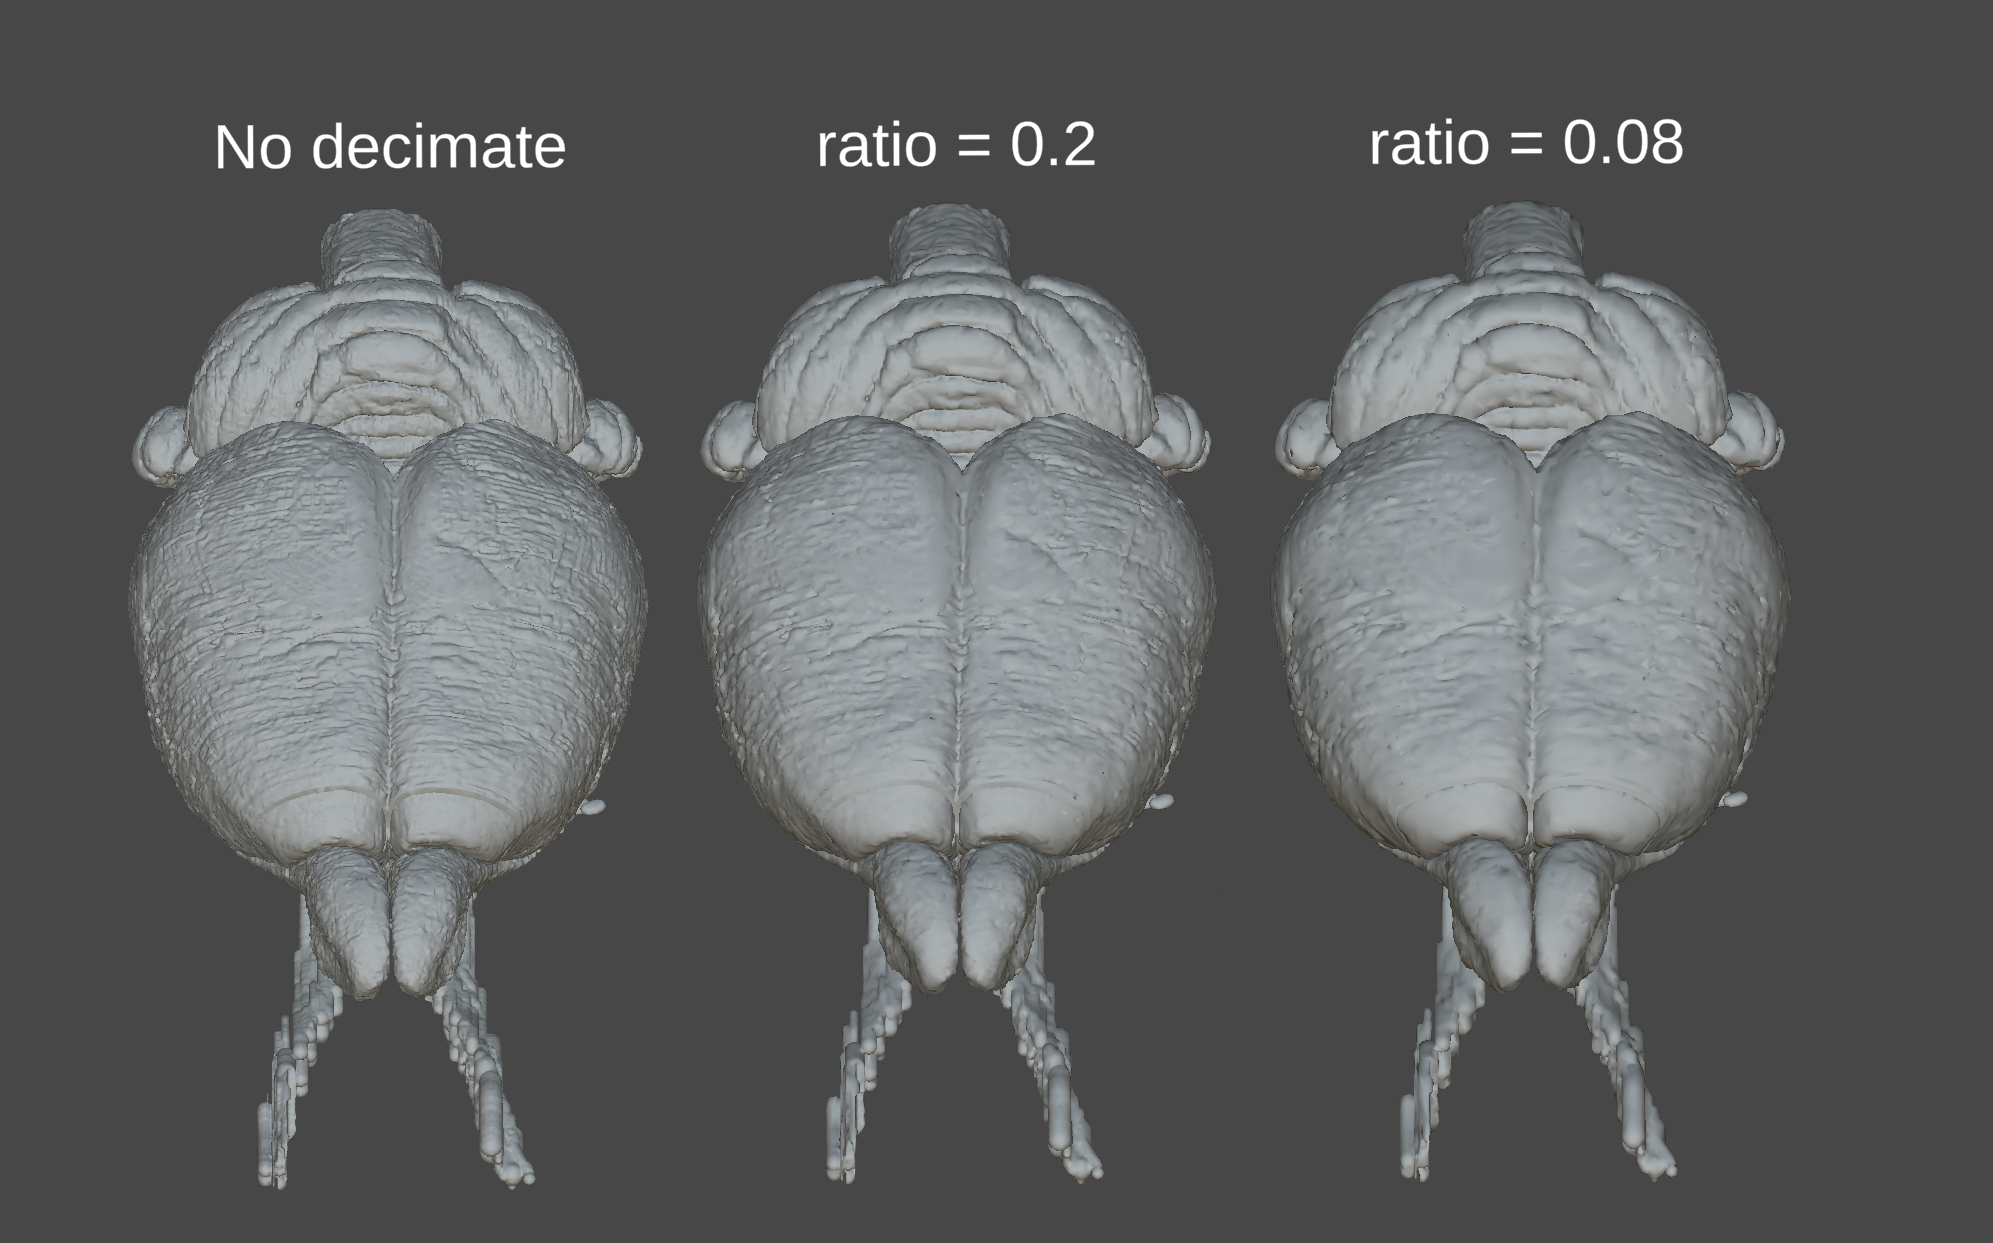
\includegraphics[width={\textwidth},trim={2.5cm 2cm 4.5cm 2cm},clip]{fig/brainmodeldecimateratio2.png}
    \caption{WHS brain models with 3M, 744K and 297K polygons respectively.}
    \label{fig:decimate}
\end{figure}



\section[Iteration 1]{First iteration: Minimum Viable Product}\label{chap:itr1}

Having a surface model of the brain running reasonably well on the HoloLens 2, the next step in developing the application was to implement basic AR-based interact features. The brain model consist of an empty parent object with 29 children each containing the mesh of a delineated brain structure, see \autoref{fig:brainunitytree}. Adding the \texttt{Object Manipulator} component from MRTK and a standard Unity \texttt{Mesh Collider} component to each child in the brain model allows for picking apart the brain. This is done by grabbing and moving each separate structure with a MRTK defined \textit{pointer}, this is the logical abstraction for the simplest interact handling with HoloLens 2 giving the user a virtual laser pointer from their finger. The resulting action can be seen in \autoref{fig:grabbrain}. 

% \begin{wrapfigure}{r}{0.38\textwidth} 
%     \centering
%     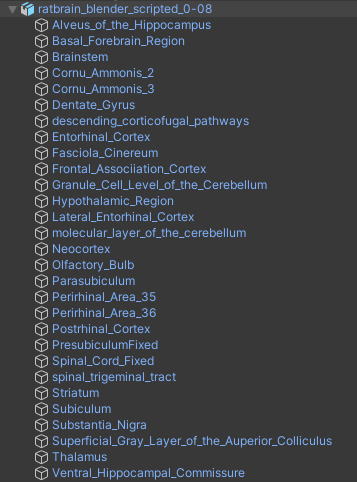
\includegraphics[width=0.35\textwidth]{fig/brainunitytree.png}
%     \caption{The tree structure of the Unity \texttt{GameObject} of the brain model.}
%     \vspace{-10pt}
%     \label{fig:brainunitytree}
% \end{wrapfigure}

\begin{figure}[ht]
    \centering
    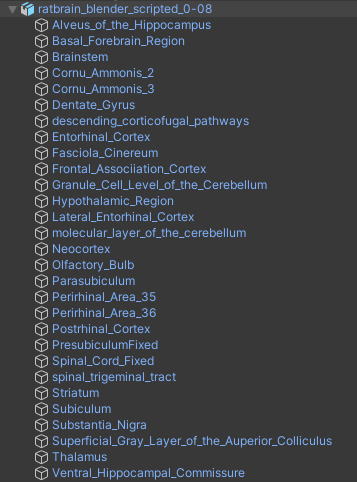
\includegraphics[width=0.30\textwidth]{fig/brainunitytree.png}
    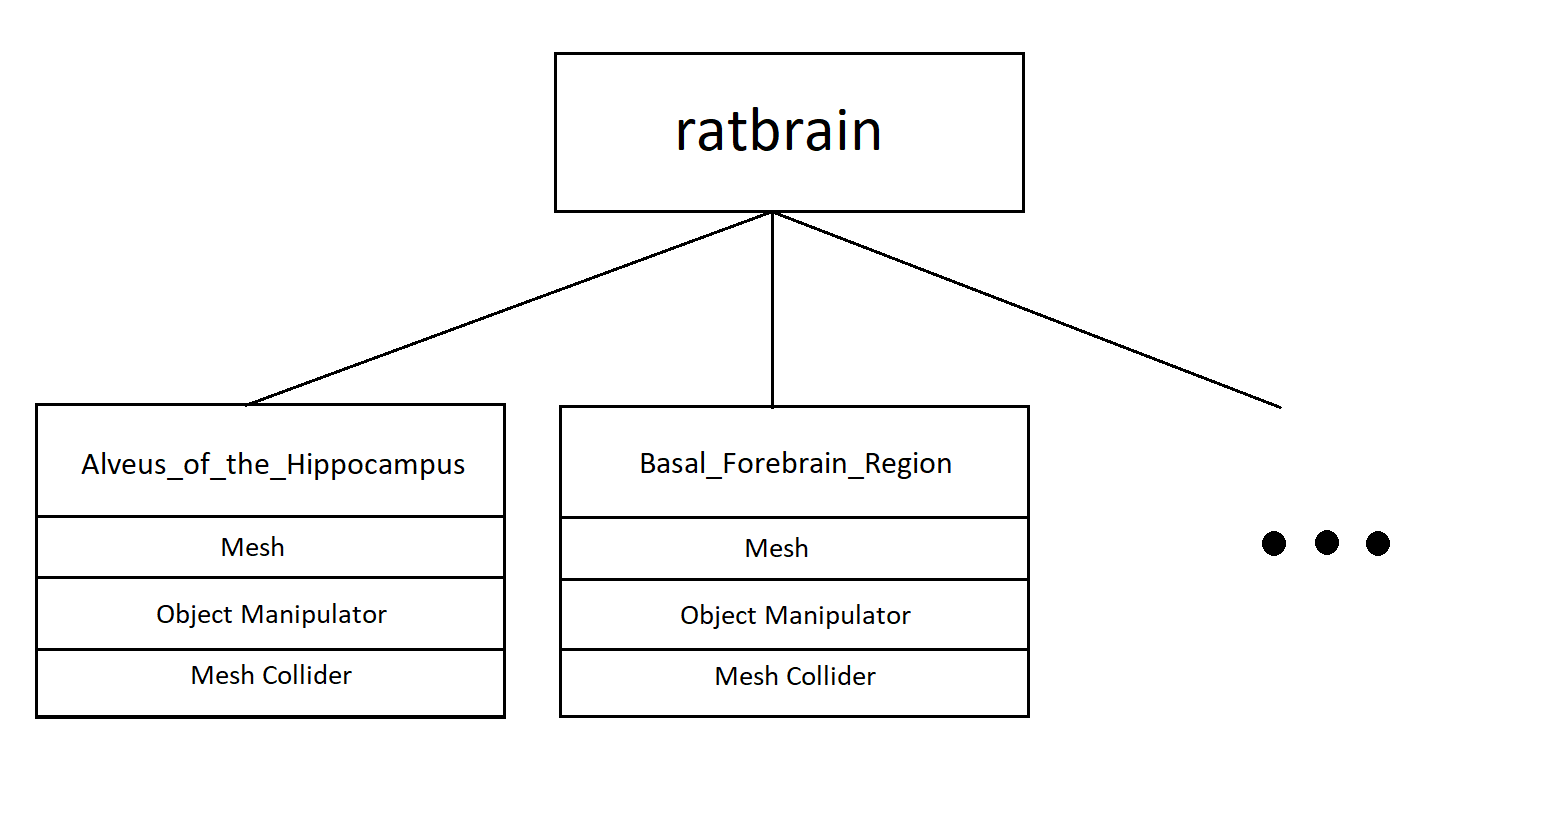
\includegraphics[width=0.60\textwidth]{fig/shittyassbraintreediagram.png}
    \caption{The tree structure of the Unity \texttt{GameObject} of the brain model.}
    \label{fig:brainunitytree}
\end{figure}

\begin{figure}[ht]
    \centering
    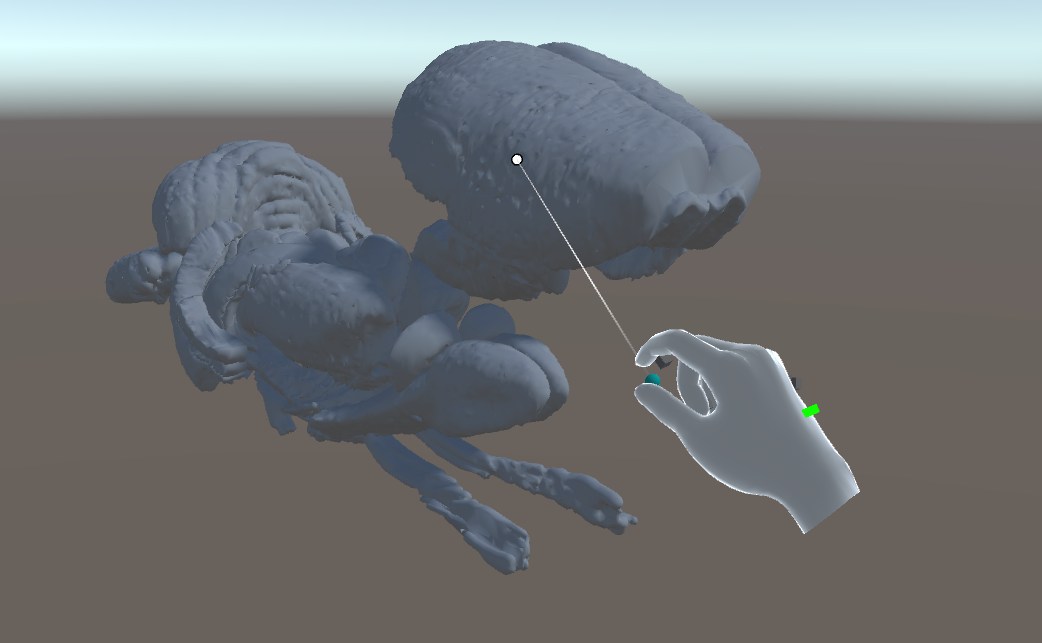
\includegraphics[width=0.8\textwidth]{fig/grabbrainsection.png}
    \caption{Grabbing the neocortex brain structure with a MRTK pointer in the Unity editor.}
    \label{fig:grabbrain}
\end{figure}

An apparent problem at this stage was that thought the brain structures are separate objects, they were difficult to visually distinguish from each other. A script which took all child objects and applied a random color to each was written and placed on the parent object, thus quickly giving some visual separation of the structures. While implementing this feature, the \textit{material} of each child was changed from Unity's default material to a \textit{MRTK Standard} material. Materials are the way Unity handles rendering details for each object, this is where shader, texture and general rendering options are configured. The MRTK Standard materials is a set of materials using the the \texttt{MixedRealityStandard.shader} shader, this shader is optimized for MR use, and superficially for HoloLens, and is meant for fulfill all shader-needs when developing for these platforms. 

% Jeg heter Ole og jeg har liten tiss

With a some basic visibility and manipulation features for the brain model, the next natural step was tackling the system requirements, specifically the first functional requirement, implementing brain dissection. A \textit{clipping} shader was written and implement to work with the brain, giving more control over the feature than using MRTKs prebuild clipping feature, but seeing as it was not possible to combine a custom shader with MRTK optimizes feature set for AR rendering, the custom clipping implementation was abandoned in favor of MRTK, using the aforementioned MixedRealityStandard shader. Clipping has the effect of removing vertices by some defined function, and by using a prebuilt clipping plane prefab and declare on which meshes is should act, a dissection affect was created. A handle for manipulating the plane was added for ease of use, by dragged a ball the plane would move such that it was a fixed distance from the ball and perpendicular to the line between the ball and the center of the brain. 


Further, a hovering menu displaying the name of the last grabbed brain structure and buttons for the actions moving, transparency and dissection was implemented. This was created by modifying a MRTK prefab and updating its name based on the name of the \texttt{GameObject} the \texttt{pointer} targeted while dragging, at the same time a selection lighting effect as applied by simply enabling \texttt{Border Lighting} in the MixedRealityStandard shader. Unity's layer functionality was used to ensure that it was a brain structurer being dragged. One last feature implemented at this phase was a tap-to-spawn feature, this entailed using the \texttt{pointer} to tap on the physical space, and using spatial awareness to place the brain at the locations the the user tapped. In MRTK spatial awareness is enabled by default and its mesh can be identified by a predefined Unity layer, thus \autoref{item:sudopointer} shows a simplified implementation of the \texttt{EventHandler} method, \texttt{OnPointerDown} which spawns the brain if the pointer is hitting the spatial awareness mesh and enables border lighting and menu text if it hits a brain structure.

\begin{lstlisting}[language=c, label={item:sudopointer}, caption={A simplified version of the event function called when a \texttt{Ponter} is clicked.}]
void OnPointerDown(MixedRealityPointerEventData eventData)
{
    if (!HasTarget(eventData.Pointer)) 
        return;
    Vector3 hitPoint = GetHitPoint(eventData.Pointer);
    GameObject target = GetCurrentTarget(eventData.Pointer);

    switch (target.layer)
    {
        case SpatialAwarenessLayer:
        {
            if (BrainHasNotBeenSpawned())
                SpawnBrainAt(hitPoint);
        }
        case BrainStructureLayer:
        {
            if (selectedStructure != null)
                DisableBorderLighting(selectedStructure);
            EnableBorderLighting(target);
            SetMenuText(target.name);
            selectedStructure = target;
        }
    }
}
\end{lstlisting}

The application was deployed for HoloLens 2, and was a first MVP demo of the research project. \autoref{fig:mvpdemo} shows spawning of the brain model from image 1 to image 2 in the top row, notice the pointer on the table in image 1. Image 3 illustrates the clipping feature, while image 4 has a user taking out the \textit{cornu ammonis 3} brain structure.

\begin{figure}[h]
    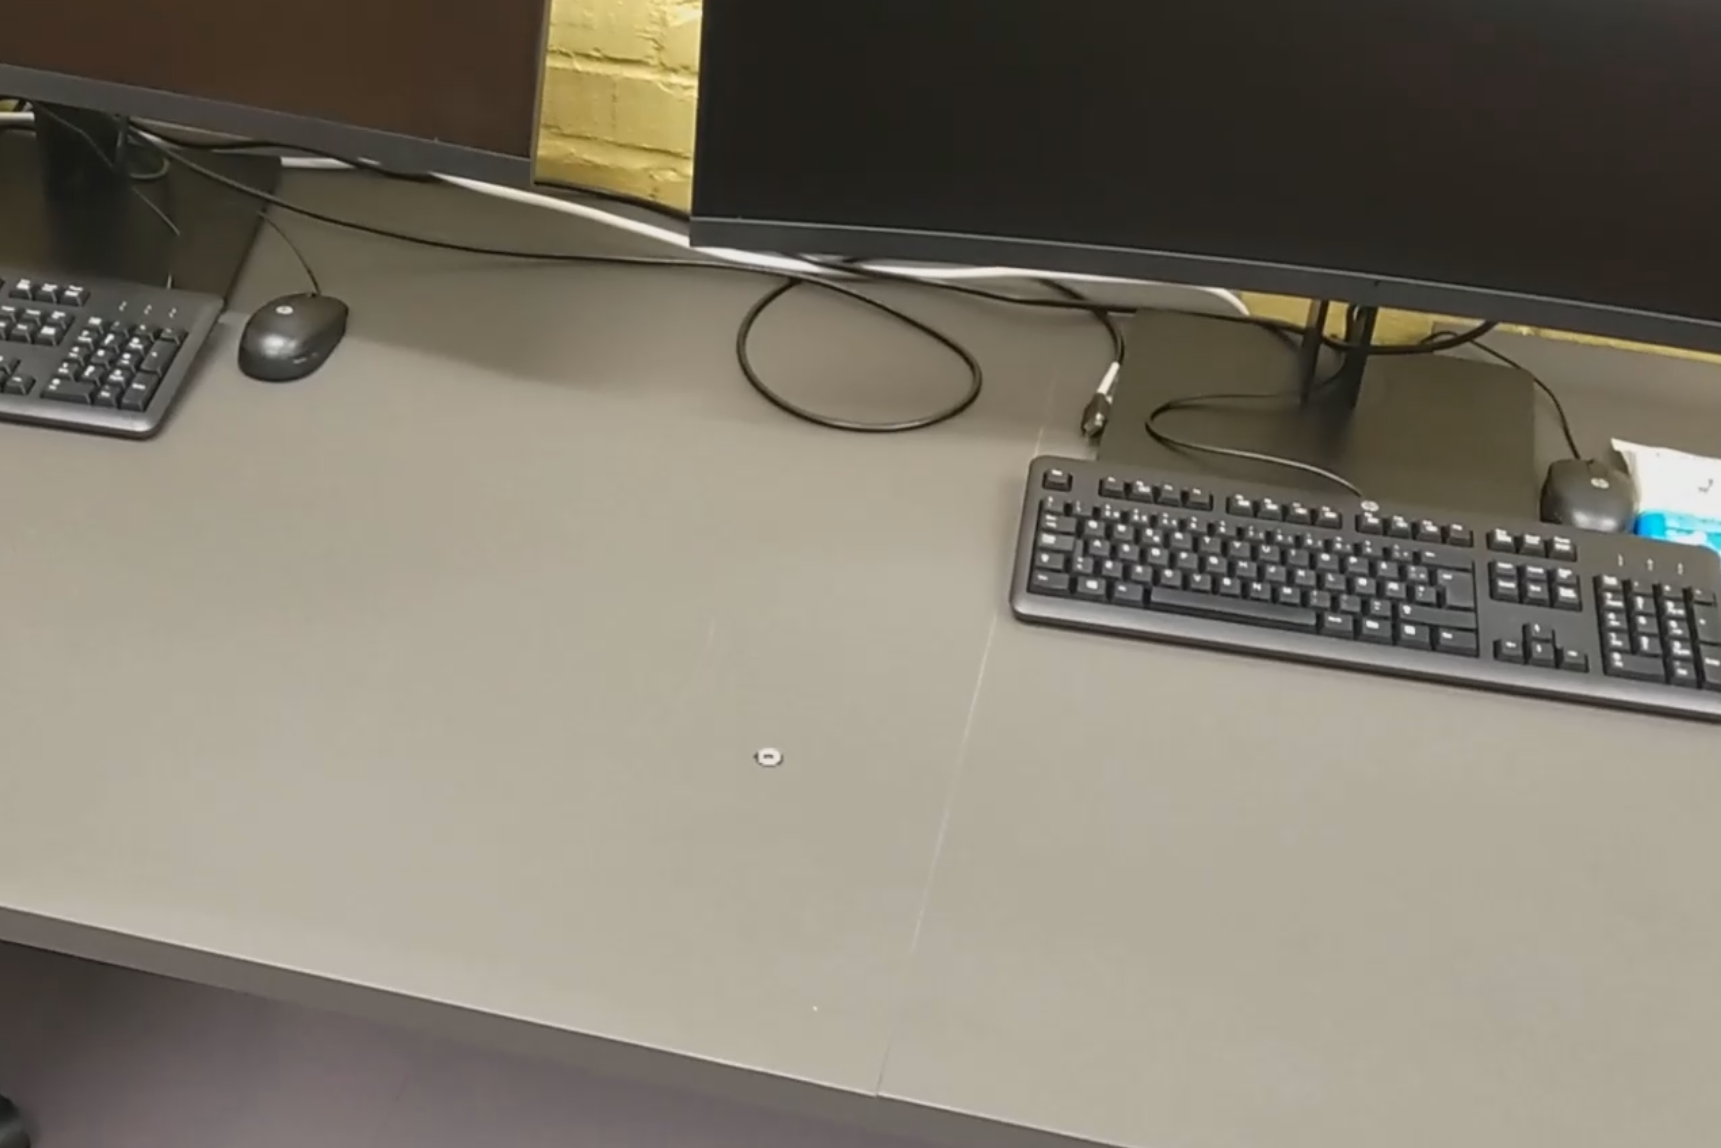
\includegraphics[width=0.5\textwidth]{fig/mvpdemo1.png}
    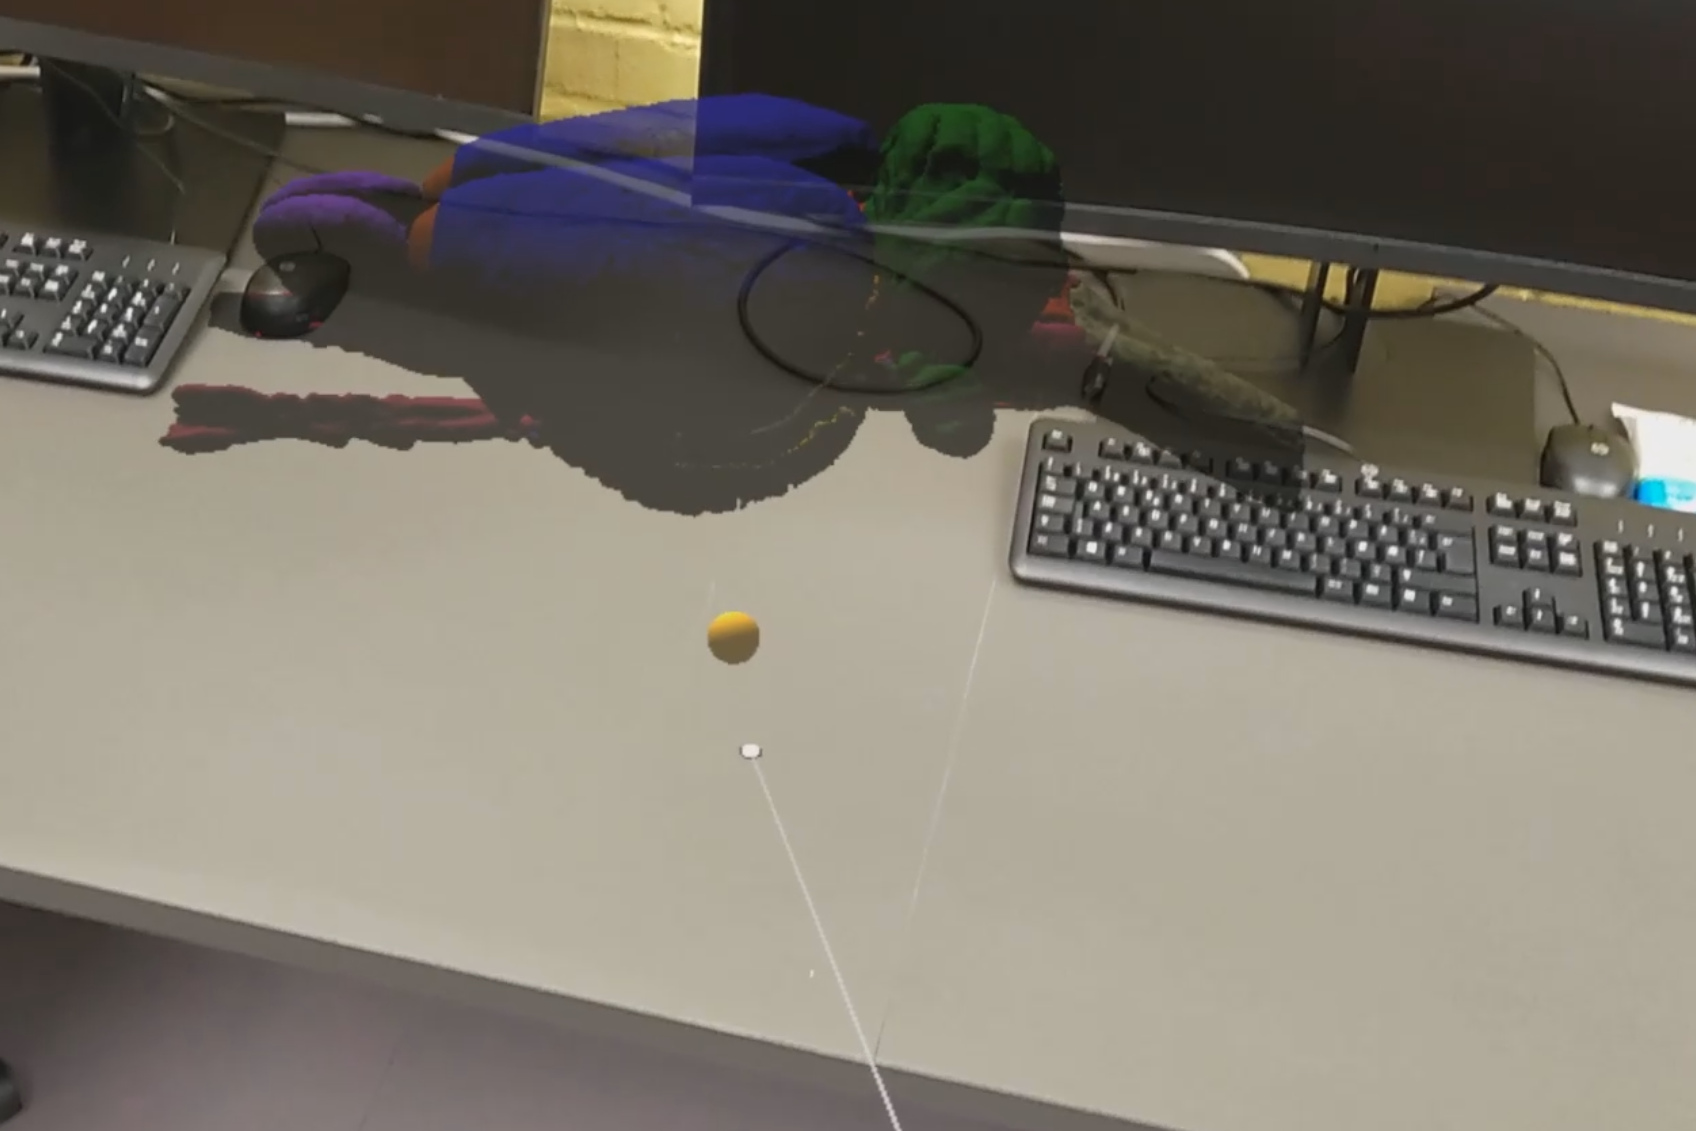
\includegraphics[width=0.5\textwidth]{fig/mvpdemo2.png}
    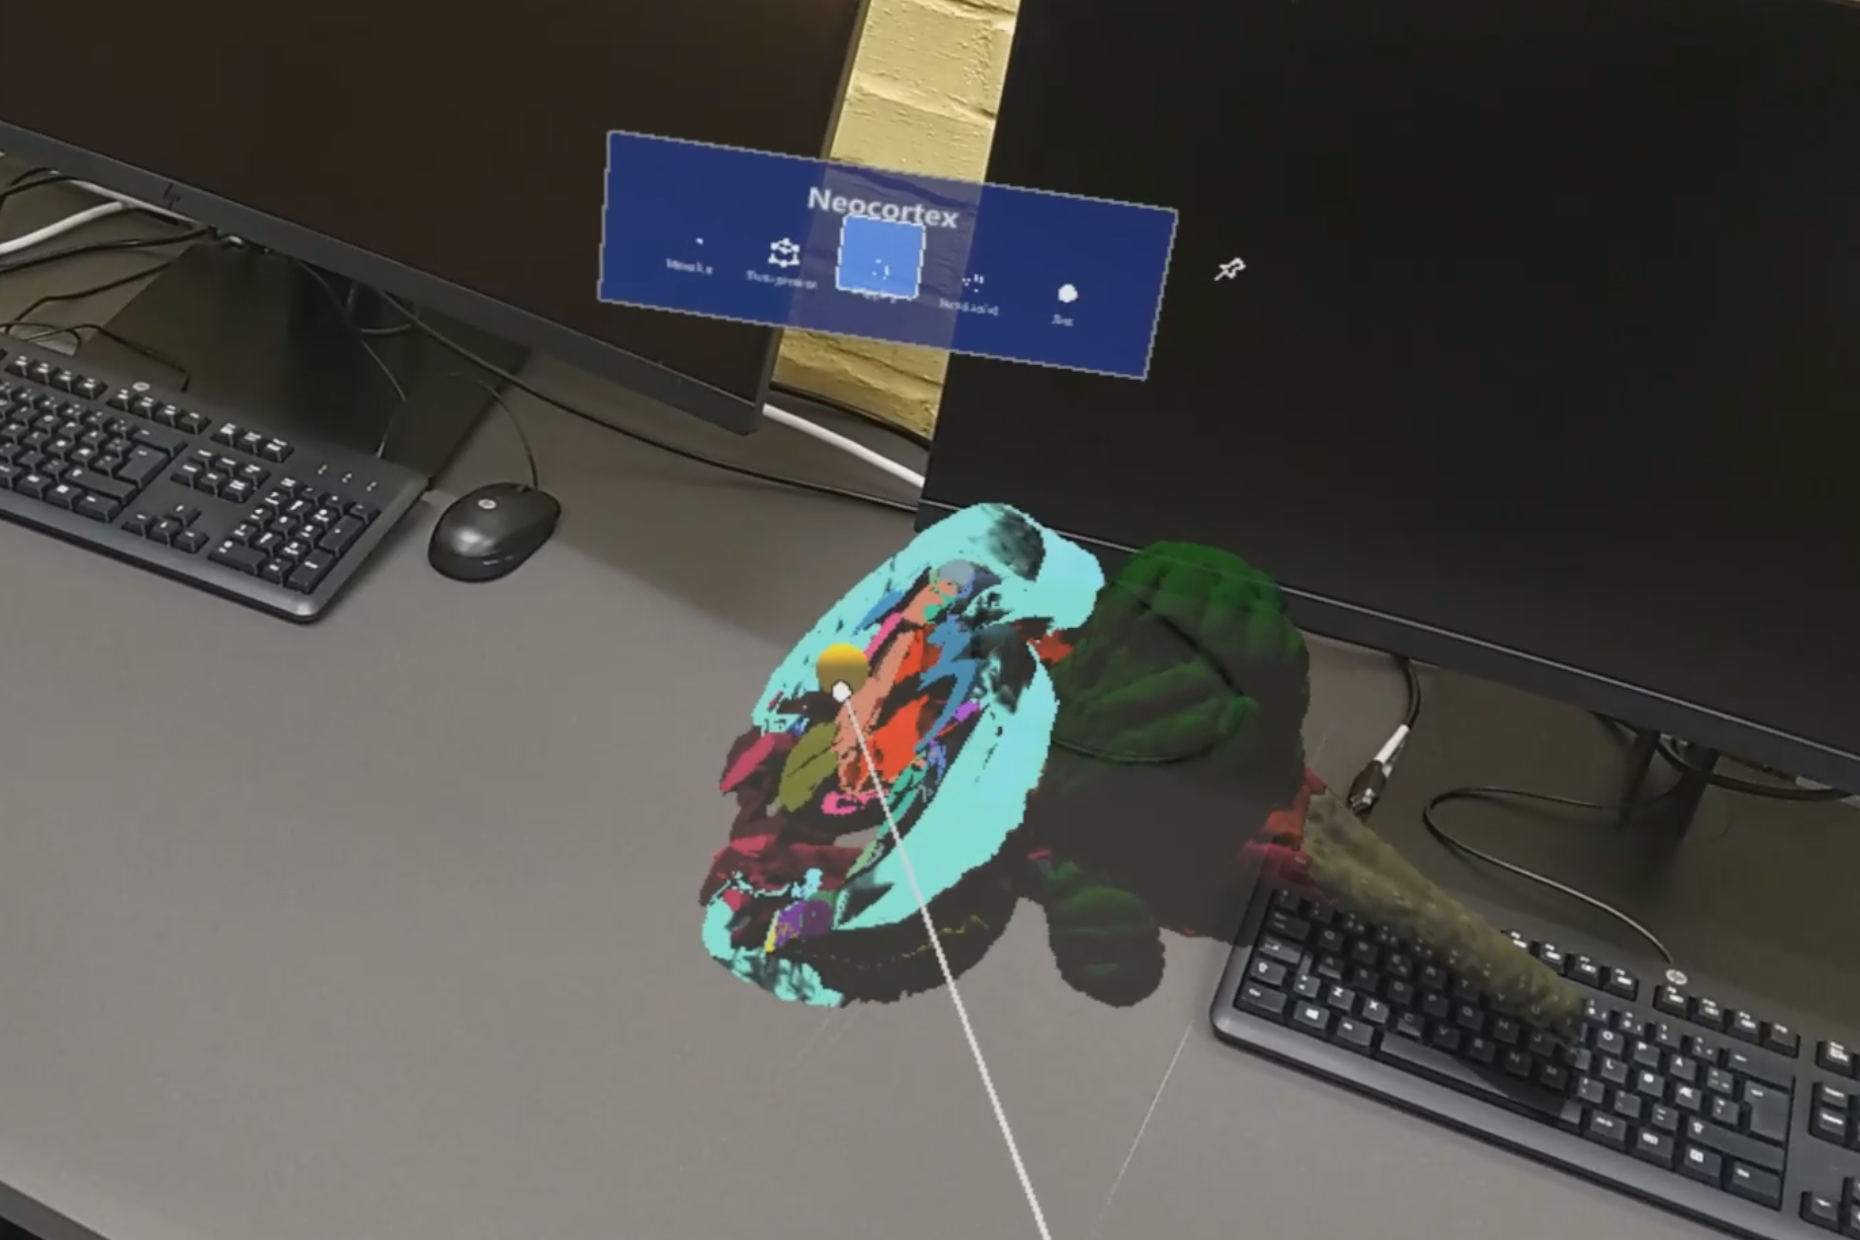
\includegraphics[width=0.5\textwidth]{fig/mvpdemo3.png}
    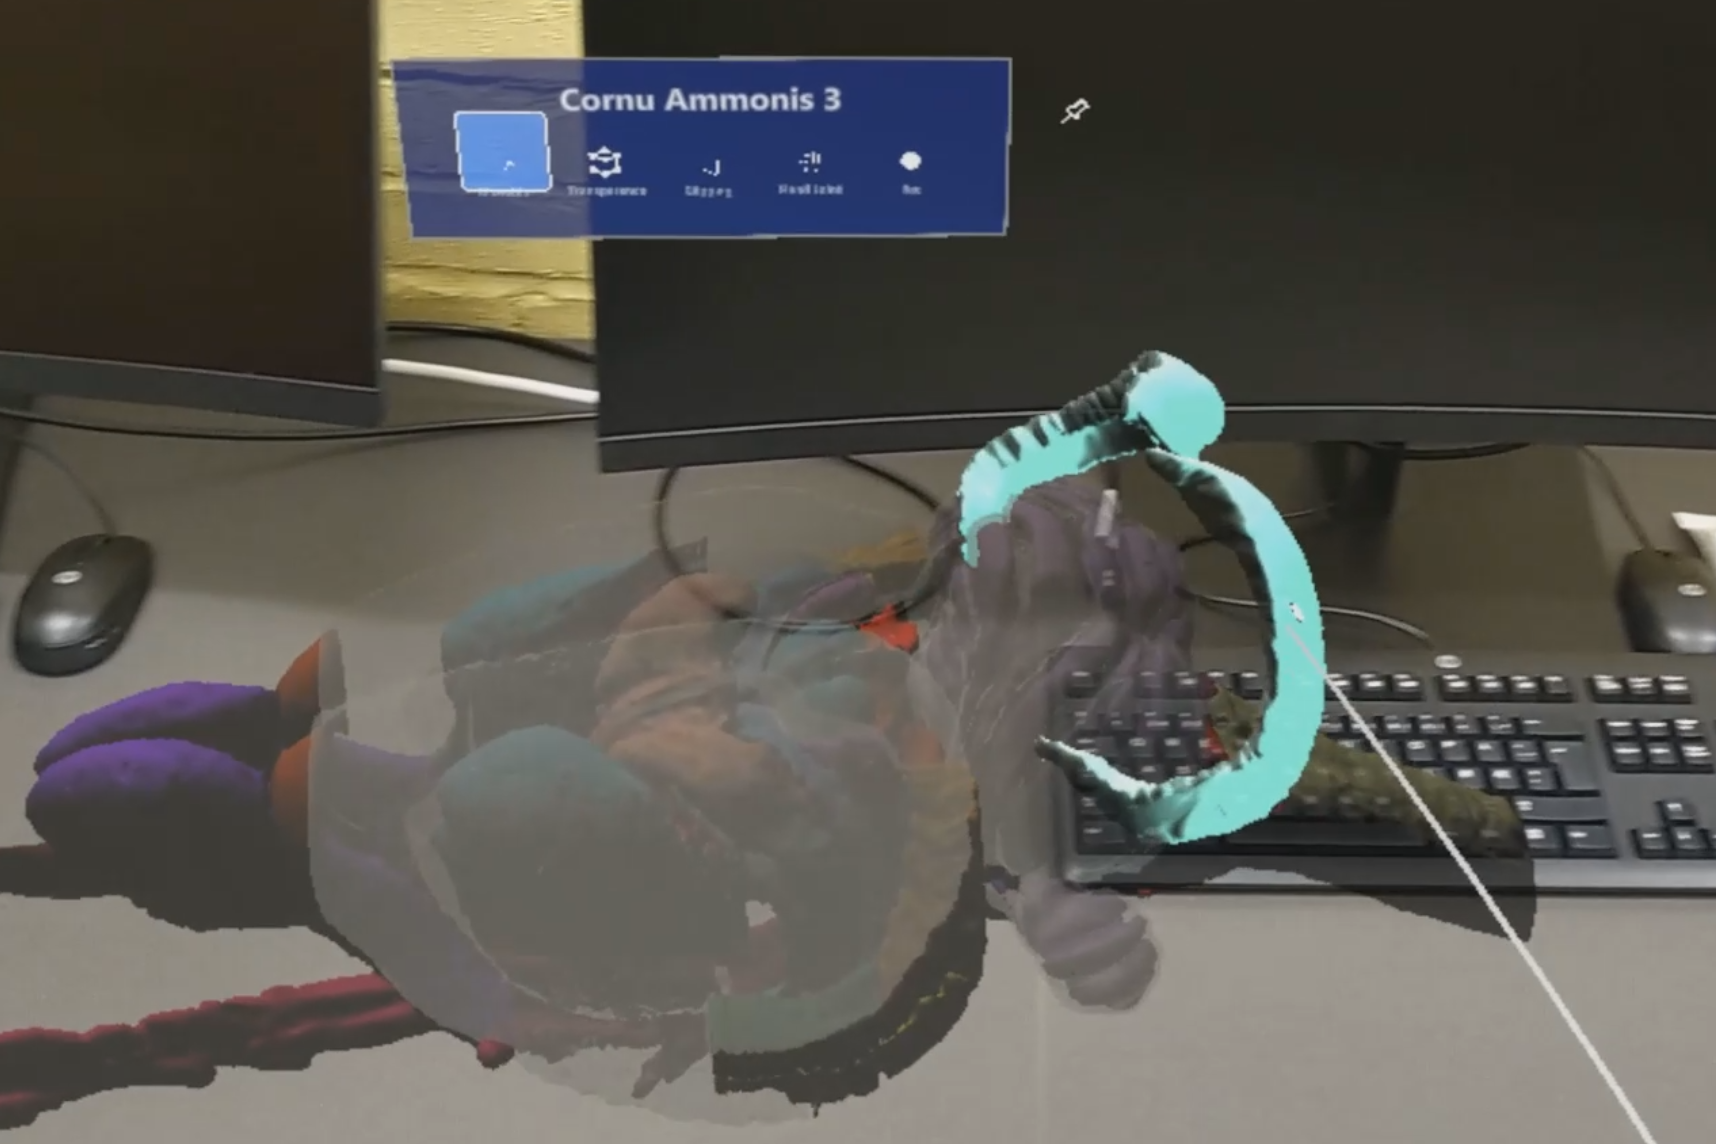
\includegraphics[width=0.5\textwidth]{fig/mvpdemo4.png}
    \caption{The first demo of the application, running on the HoloLens 2.}
    \label{fig:mvpdemo}
\end{figure}

\section[Iteration N]{Next iterations: Continuing development}

The continuation of the project will be explored further, but will focus on implementation of highlighted features and and high-level overview of the process, rather than a chronological log as in previous sections. 
% This section will give a overview of the continued progress in developing the application and highlighting some specific features. 

Shortly after end of the first iteration a demonstration of the application was done over video conference, with a pre-recorded YouTube video, demonstrating the features of the application. In addition a physical stakeholder meeting at St. Olavs Hospital was arranged where only the project researcher used the application with the HMD, but through live streaming the video feed from the headset and operational guidance from Dr. Menno Witter testing of dissection features were held. The application was at this stage nearly identical to what was seen at the end of the \nameref{chap:itr1}, with minor tweaks and bug fixes.

After this initial demonstrations stakeholders from the Kavli Institute were intrigued to see further development and had very positive sentiments toward the research project. Feedback gathered from this meeting included mainly two features, an ability to place brain structures back into the brain after deconstruction, basically to tidy up the brain after manipulation. Second, a list view for choosing which brain structures should be visible, this feature request was inspired by Eldens \nameref{chap:vrvis} which some of the stakeholders had previous experience with.

\subsection{Snapping}
The first of the described feature request to be able to put brain structures back into place. Snapping structures as magnets was suggested as a metaphor for the action. 

This snapping effect was implement as a \texttt{MonoBehavior} called \texttt{SnapInPlace}, by storing the \texttt{initialPosition} of each snappable object and comparing the distance to this position with a given \texttt{threshold} distance at the end of each manipulation: 

\begin{lstlisting}[language=c]
void OnManipulationEnded() {
    if (Distance(initialPosition, structure.position) < threshold) 
        // set brain structure to initial position 
        structure.position = initialPosition; 
}
\end{lstlisting}

This worked as expected, however no indication of the snapping behavior was given to the user and so it could be interpreted as an unexpected behavior when the brain structure just disappears when the user releases it. This issue was solved by having a semi-transparent shadow of the brain structure at its initial position colored green when snapping would occur at release and gray otherwise. Additionally, a audio effect was implemented such that a clicking sound as the structure snapping in place. 
As the snap implementation code above suggests, structures are snapped in place the same frame as the manipulating has ended. It was experienced with using \textit{lerping} for smoother movement, however it was found to not give the same feeling of "snap" as just setting the position and playing a sound effect.

\begin{figure}
    % 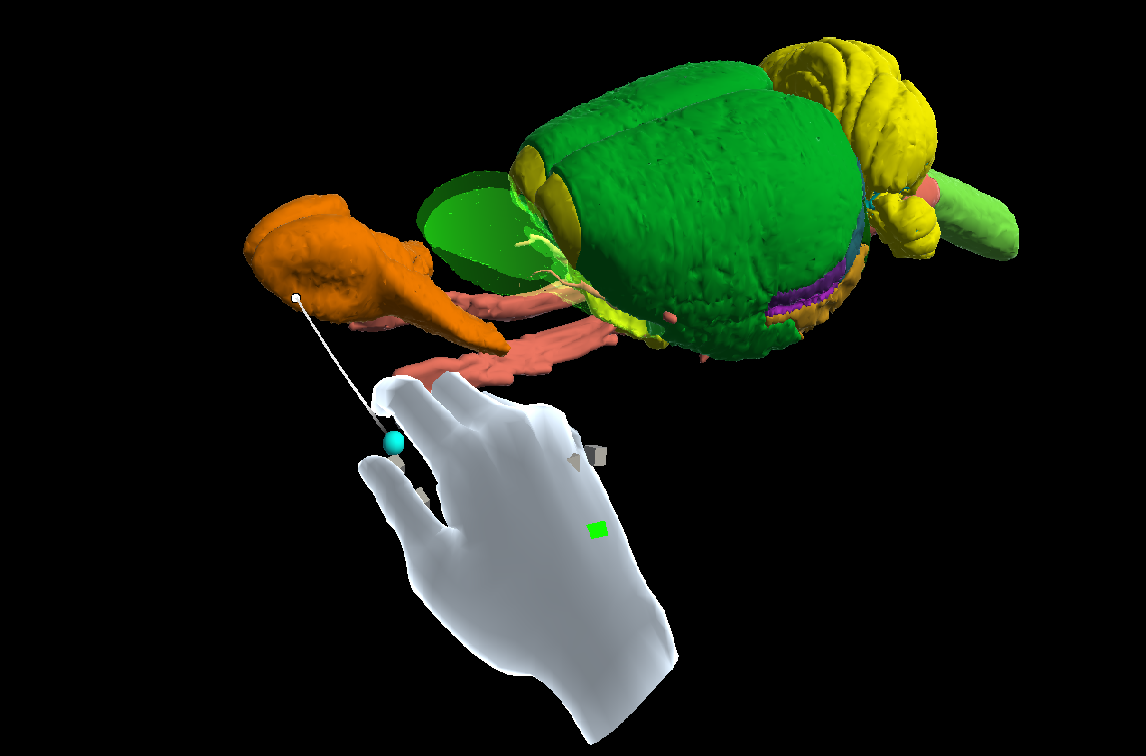
\includegraphics[width=0.65\textwidth]{fig/snaphint.png}
    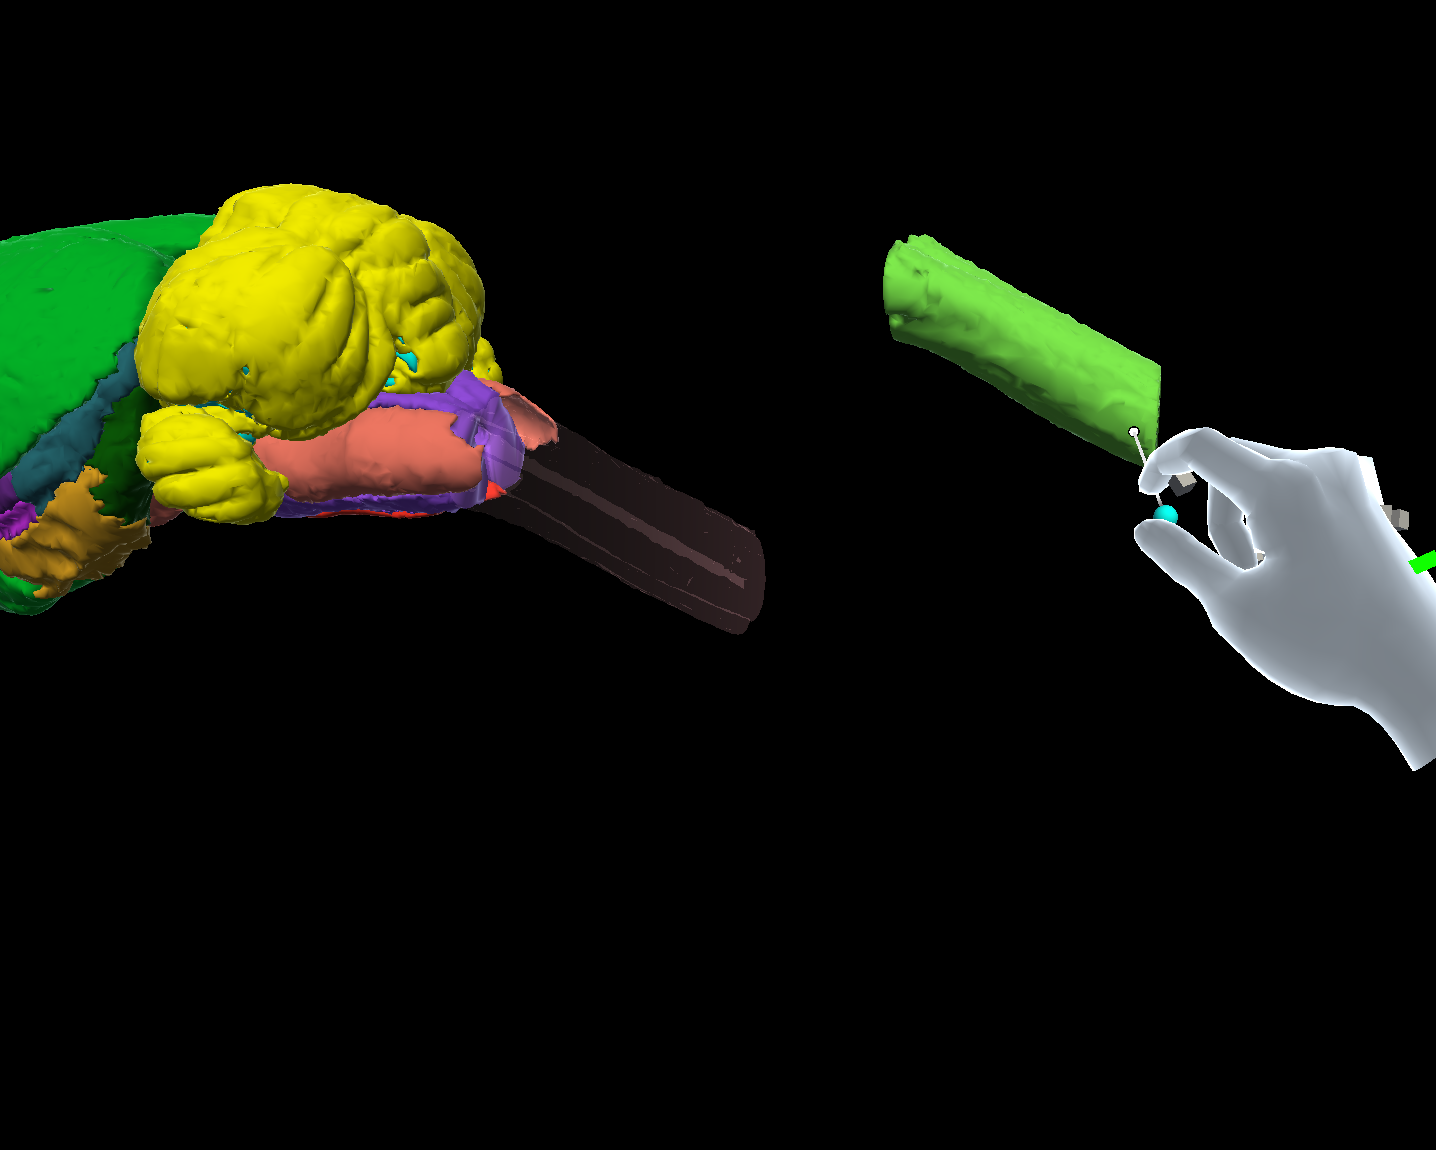
\includegraphics[width=0.33\textwidth]{fig/snaphint1.png}
    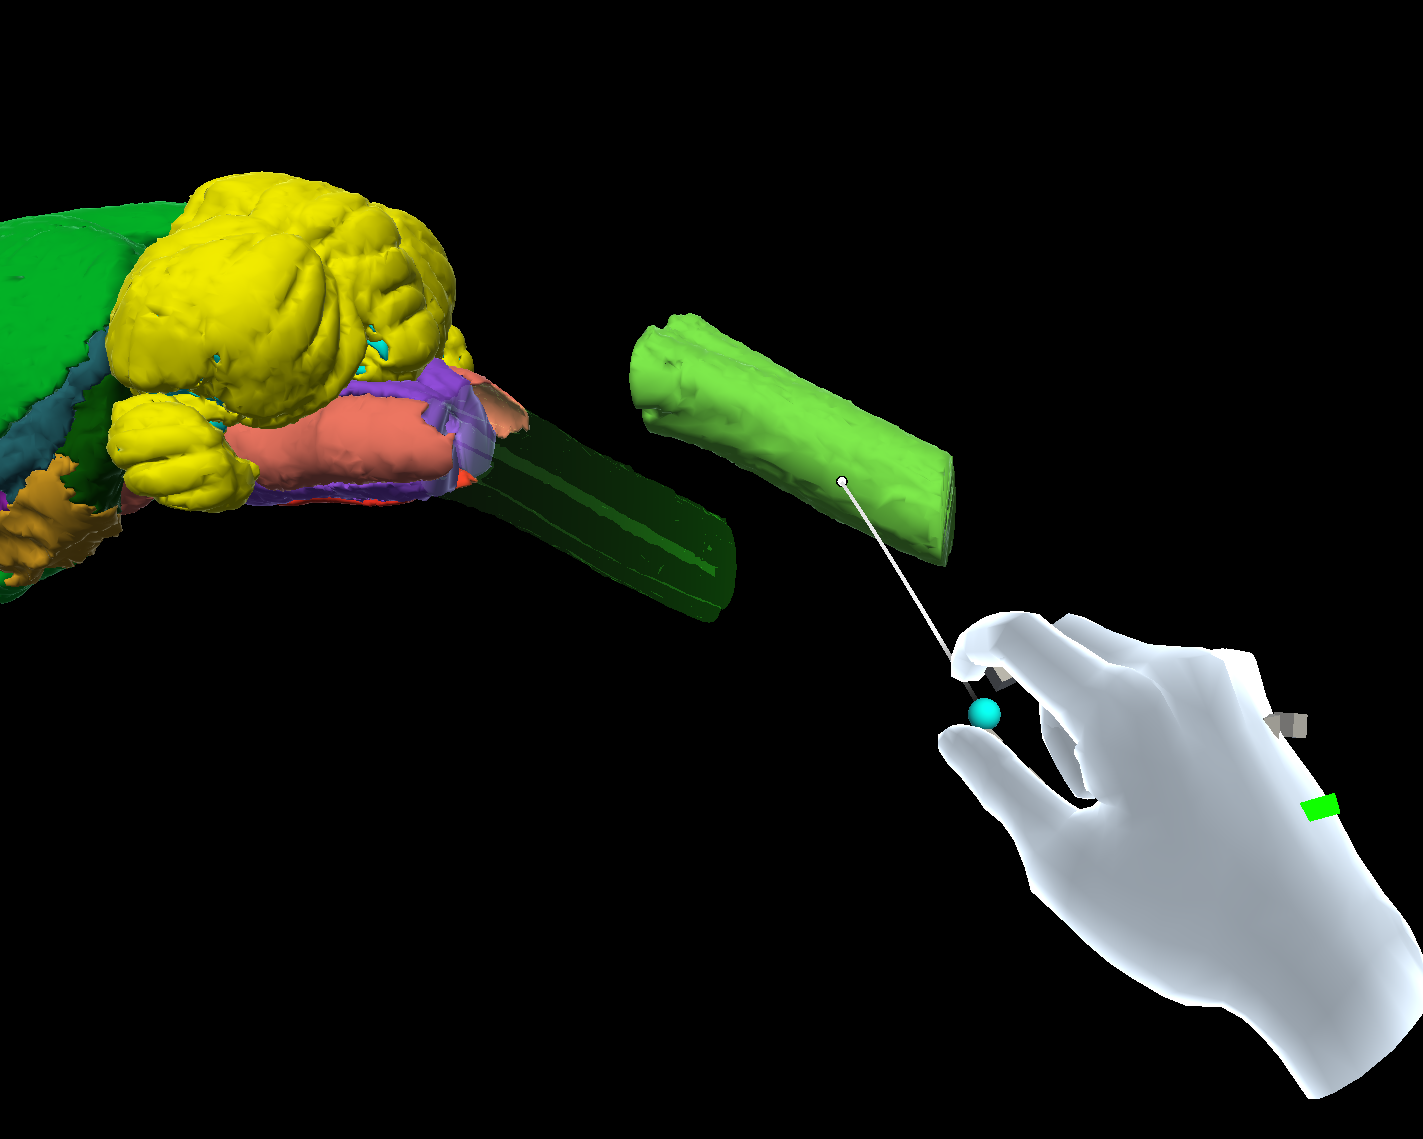
\includegraphics[width=0.33\textwidth]{fig/snaphint2.png}
    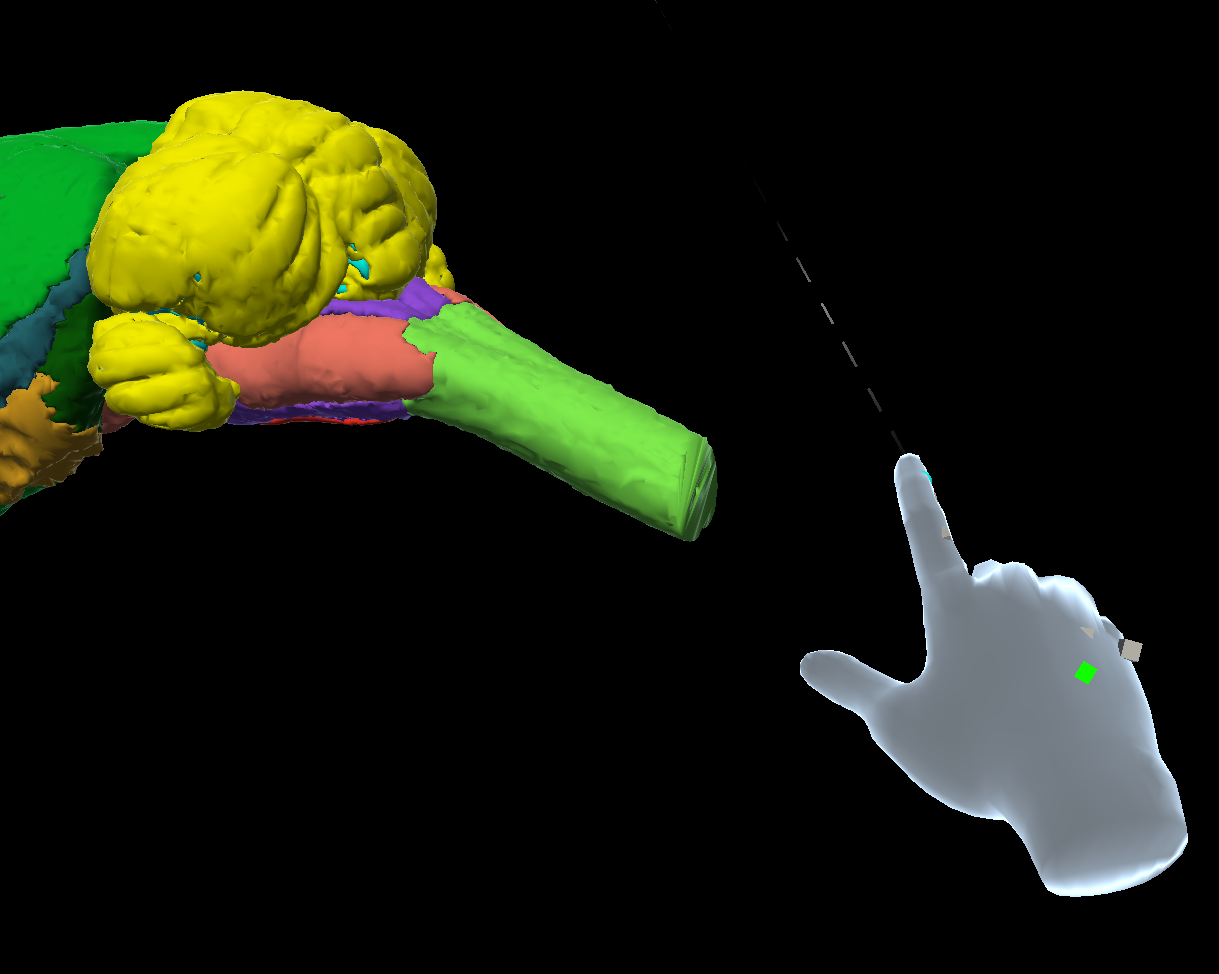
\includegraphics[width=0.33\textwidth]{fig/snaphint3.png}
    \caption{The complete snapping process. Right most image shows the brain structure snapping in place at release.}
\end{figure}

% \subsubsection*{Scrollable list view}

% A list view similar to the one in \nameref{chap:vrvis}, as seen in \autoref{fig:vrvis} was requested by stakeholders. 


\subsection{User Interface}

User interfaces in augmented reality is still a rapidly developing field with few optimal solution. This project uses quite minimal UI for simplicity of use and development, but some UI is required i.a. for enabling features and informing the user. During this project, several iterations on menu design has tried and found lacking. The first iteration is seen in \autoref{fig:mvpdemo} and is a combination of text content naming the selected brain structure and action buttons. This worked as for simple MVP purposes, but was far from optimal. It was tedious for users to click the buttons as they were hovering above the brain model. 
% \subsubsection*{Feedback from demo}
% list view

\begin{figure}[h]
    % 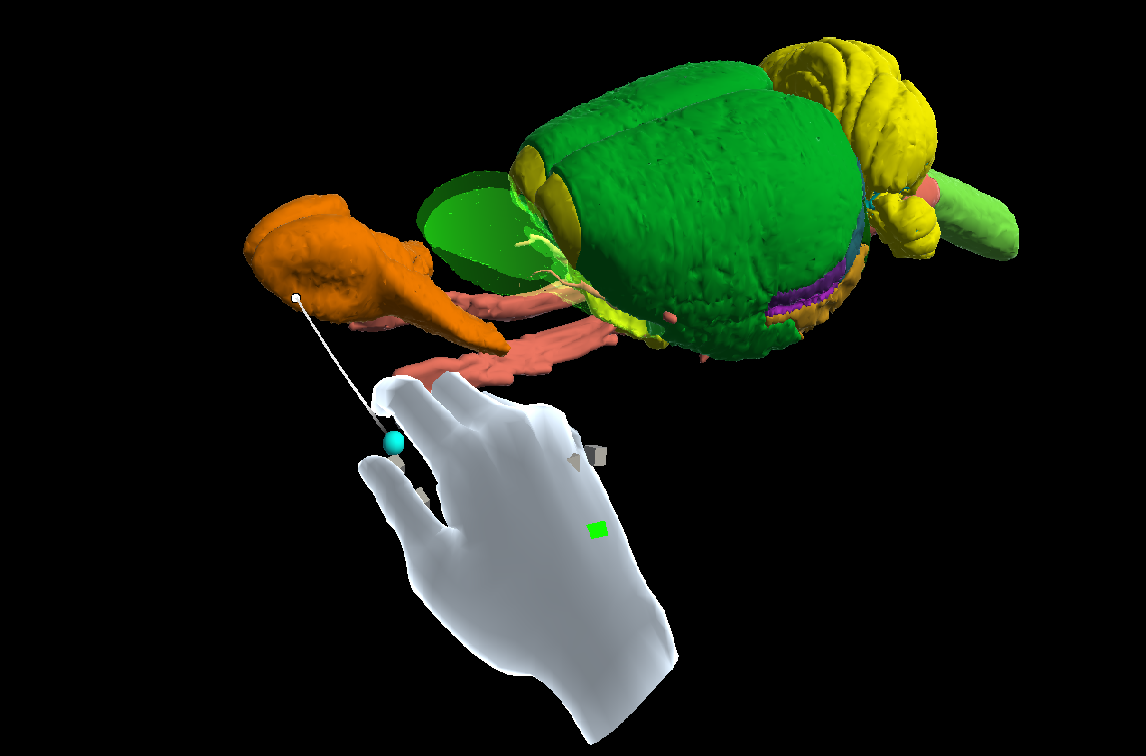
\includegraphics[width=0.65\textwidth]{fig/snaphint.png}
\begin{subfigure}[b]{0.5\textwidth}
    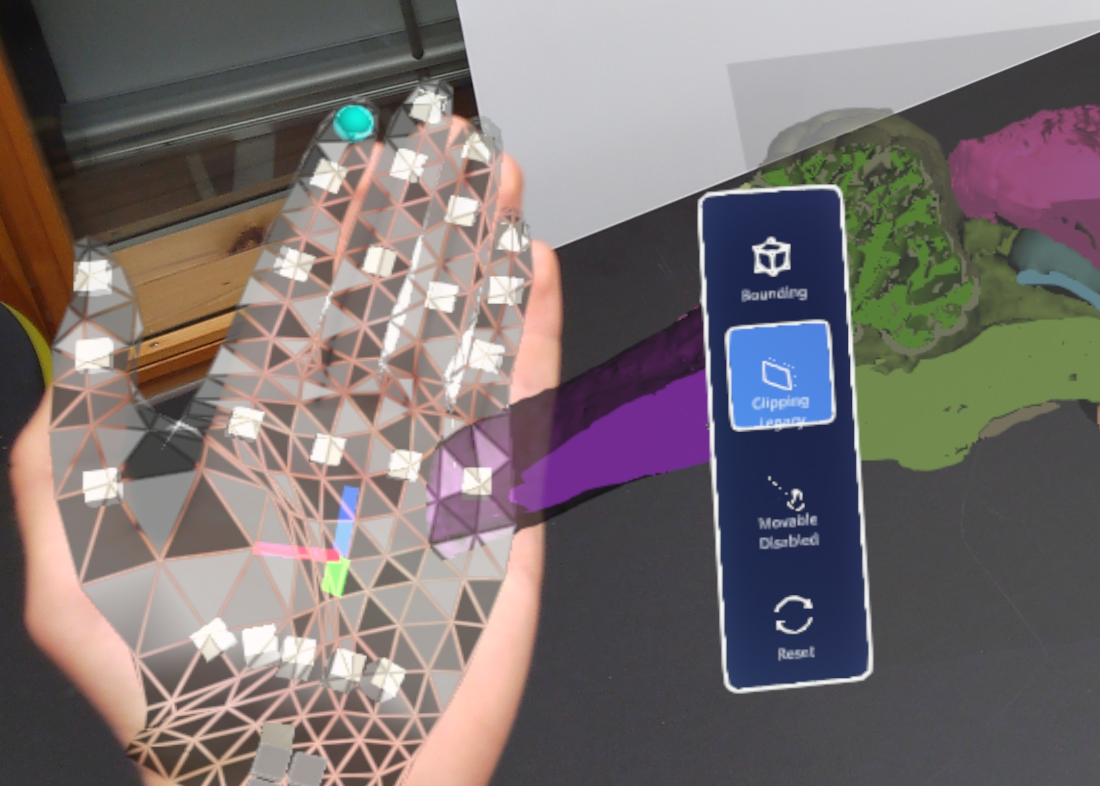
\includegraphics[width=\textwidth]{fig/handmenuiter2.png}
    \caption{Second iteration}
    \label{fig:hanmenuiter2}
\end{subfigure}
\begin{subfigure}[b]{0.5\textwidth}
    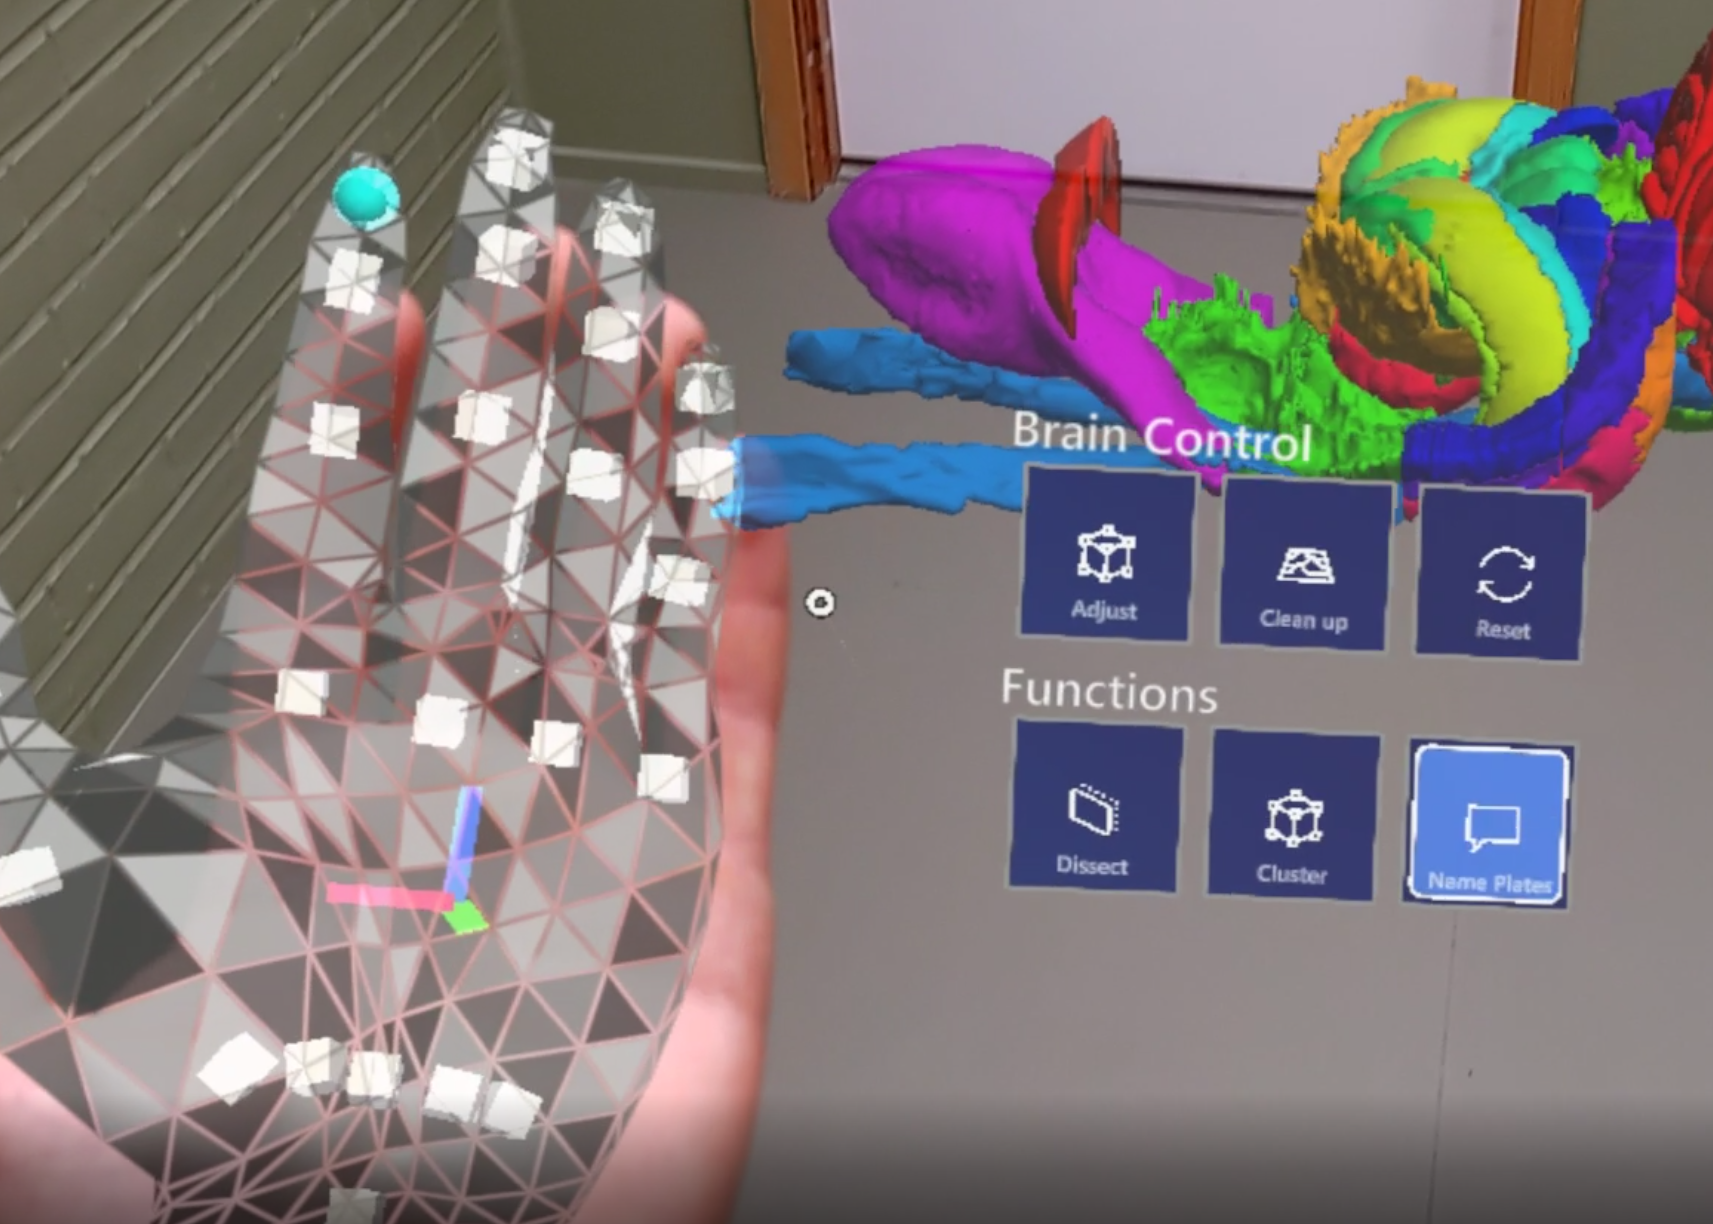
\includegraphics[width=\textwidth]{fig/handmenuiter3.png}
    \caption{Final iteration}
    \label{fig:hanmenuiter3}
\end{subfigure}
\caption{}

\end{figure}

This was solved by adding the action buttons to a menu which follows the hand of the user. This can be seen in \autoref{fig:hanmenuiter2} which uses a prefab hand menu found in MRTK. The prefab was however deemed too inflexible and a custom hand menu was designed. This new design uses default MRTK \texttt{PressableButtons} grouped by context in horizontal \texttt{GridObjectCollections}, which again are in a vertical \texttt{GridObjectCollection} that uses a \texttt{HandBound} and \texttt{HandConstraintPalmUp} component to follow the users hand. In short the menu is designed by using simpler MRTK building blocks to create a more scalable hand menu, a early version of this menu design can be seen in \autoref{fig:hanmenuiter3}. The horizontal button groups can be hidden or shown based on context, in the final product there are five button groups; \textit{Brian Control}, \textit{Tools}, \textit{Admin Tools}, \textit{Clustering Control}, \textit{Dissection Tools}. The first two will always be visible, while the rest are context aware.
Hand menus have one big issue, they are dependent on hand recognition. So devices without this feature can not fully utilize this type of UI, the solution used in this project is to simply disable the \texttt{HandConstraintPalmUp} for other device types, as in \autoref{item:androidcode}, and let the menu hover in air. This is of course wildly suboptimal, and a better cross platform solution should be implemented in further research.


\subsection{Info Board}
Textual information about the brain structures was requested by stakeholders as a educational tool for student to use by them self or in groups. The idea was that lecturers could add text as they see fit and change it to an appropriate level for the intended user group. 
This feature was implemented based on the MRTK \texttt{Slate} with is an AR based floating text box, perfect to simulate a black board. In fact, if wished for in the future it would be trivial to make it look more as a black board by changing the color and the font to something more handwritten.
The slate was customized by changing the content text reference from \texttt{InfoBoard} MonoBehavior when the a new brain structure was selected, this was done with a \texttt{UnityEvent}, a simple callback function, implemented to trigger when a new brain section is selected (this implementation
 is found in \texttt{NetworkBrainManager.cs}). The text descriptions for each structure is saved as a text file and is parsed in \texttt{InfoBoard.cs}, the text file uses a custom structure where "@" at the begin of a line indicates a new brain structure and "+" indicates a added images and and all other text is seen as descriptions for the last indicated brain structure. This works well enough, but an obviously more standard and readable approach would be to use a common text based serialization format like JSON or XML. In future development it should be looked into using one of these as both are well supported with built-in deserialization features in Unity with C\#. The implementation does not support any run-time importing of this text even though the parsing is done at run time, functional it would thus be trivial to add. What has to be implemented for this to work however is either file exploring or some other way of accessing files, e.g. from network, see \nameref{chap:futurework} for more on this.

\subsection{Clustering}\label{chap:clustering}

By clustering brain structures based on the neurological attributes lecturers can visualize how complete compound structures operation and where they are located in the brain. Just as the \texttt{InfoBoard} this feature utilizes a custom text file parser to define each clusters name, brain structures and color pallet. Again JSON or XML would probably be a wise transition for these configuration files. 
When selecting the clustering action, the \texttt{Clustering} MonoBehavior iterates through all brain structures and enables or disables according to whether it is a part of the cluster. It also assigns a new color based on the color pallet defined in the configuration file. Color pallets are defined based on HSV color hues, with two numbers indicating start and end hue in degrees, then the brain structures are assigned colors uniformly the given sector of the color wheel. This was found to be a simple and reliable solution to color coding, but could with ease be argue as not being a intuitive solution for unaccustomed or non-technical users. 
For users not to loose spatial orientation when exploring the clusters a outline of the rat brain was added. This outline is a hollow version of the geometric brain model, which was created by manually selecting all outer vertices of the brain model using Blender, this is far from a perfect approach and gives a inaccurate and rough outline and a high polygon count, however if not for future performance issues the author sees no need to fix this.


\begin{figure}[ht]
    % 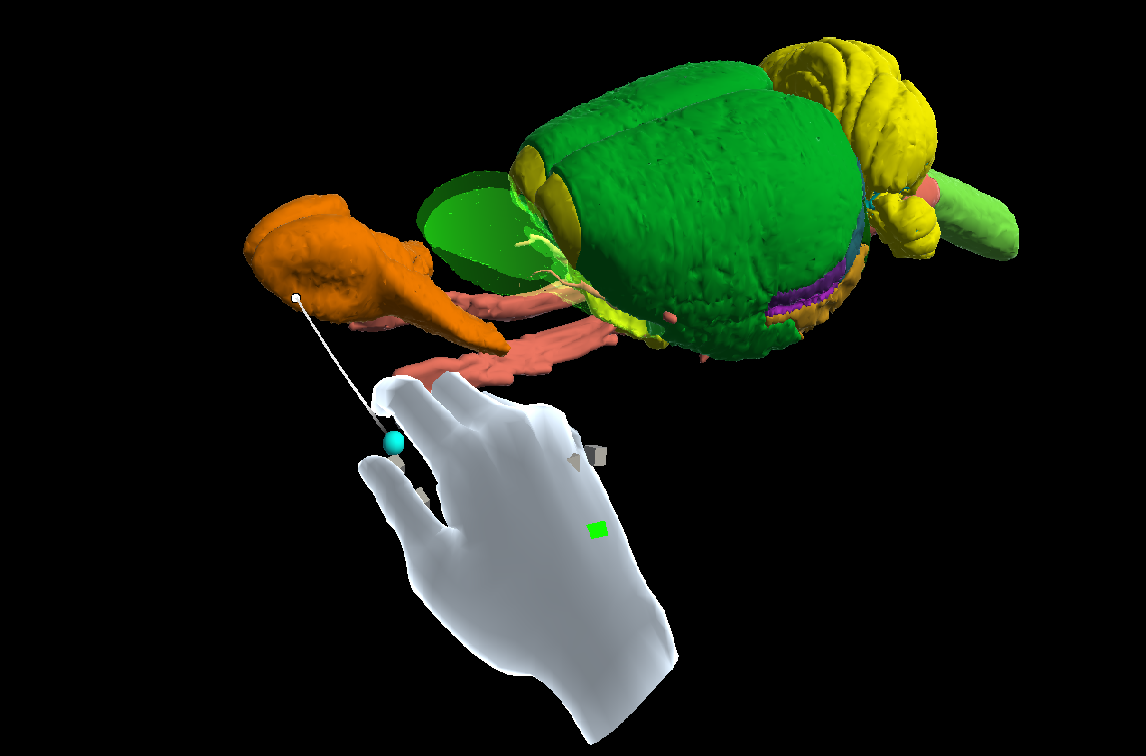
\includegraphics[width=0.65\textwidth]{fig/snaphint.png}
    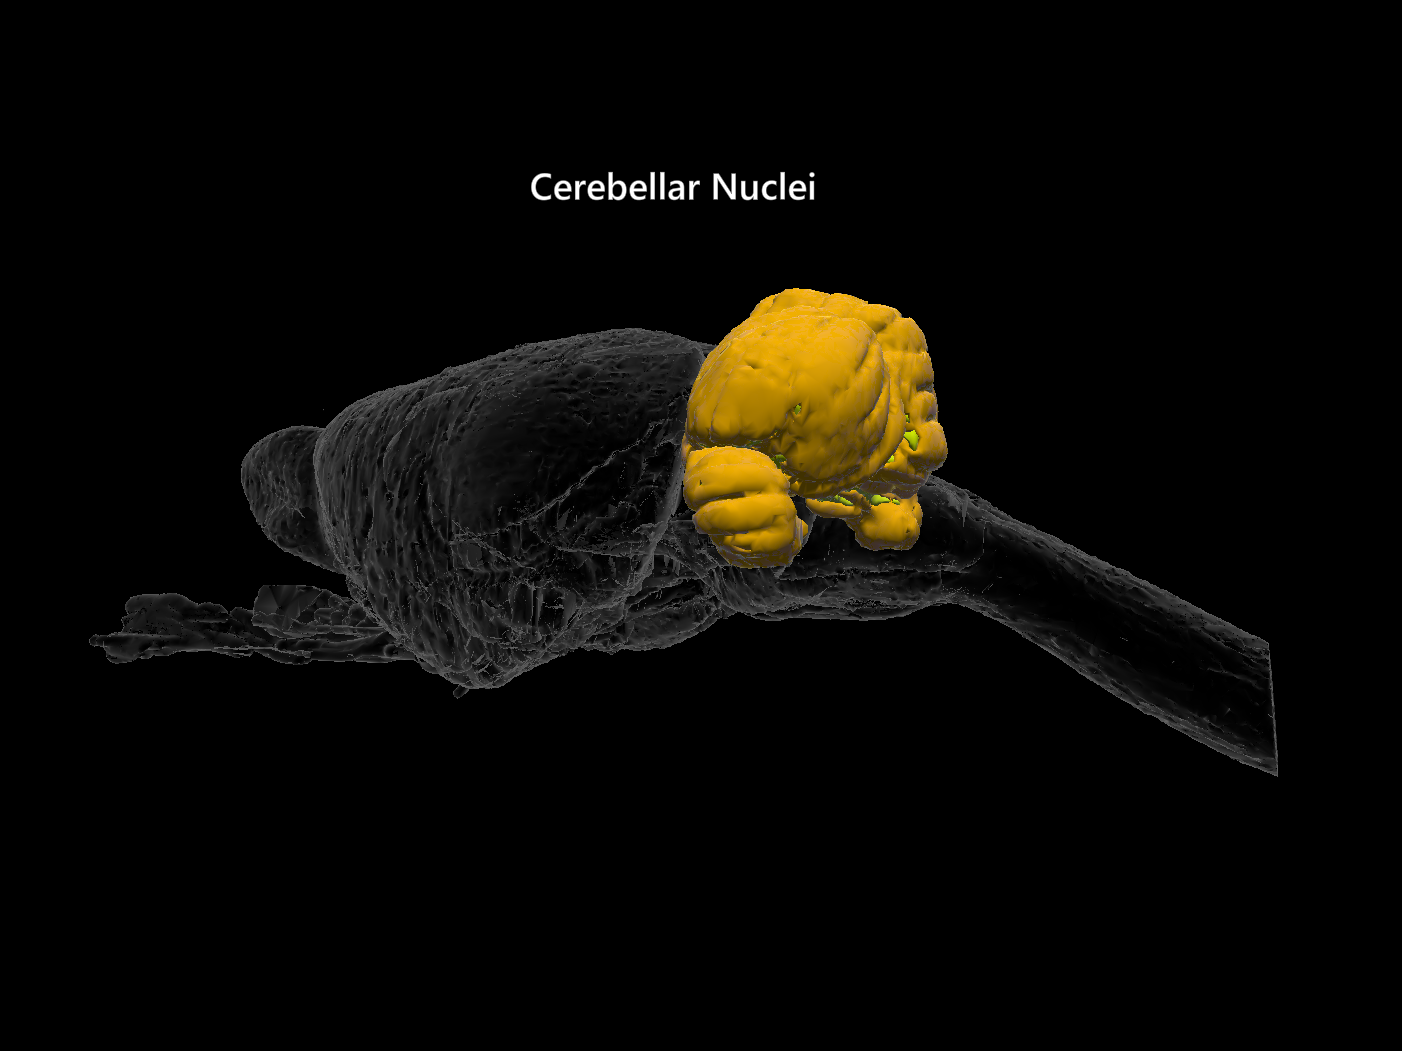
\includegraphics[width=0.33\textwidth]{fig/cluster1.png}
    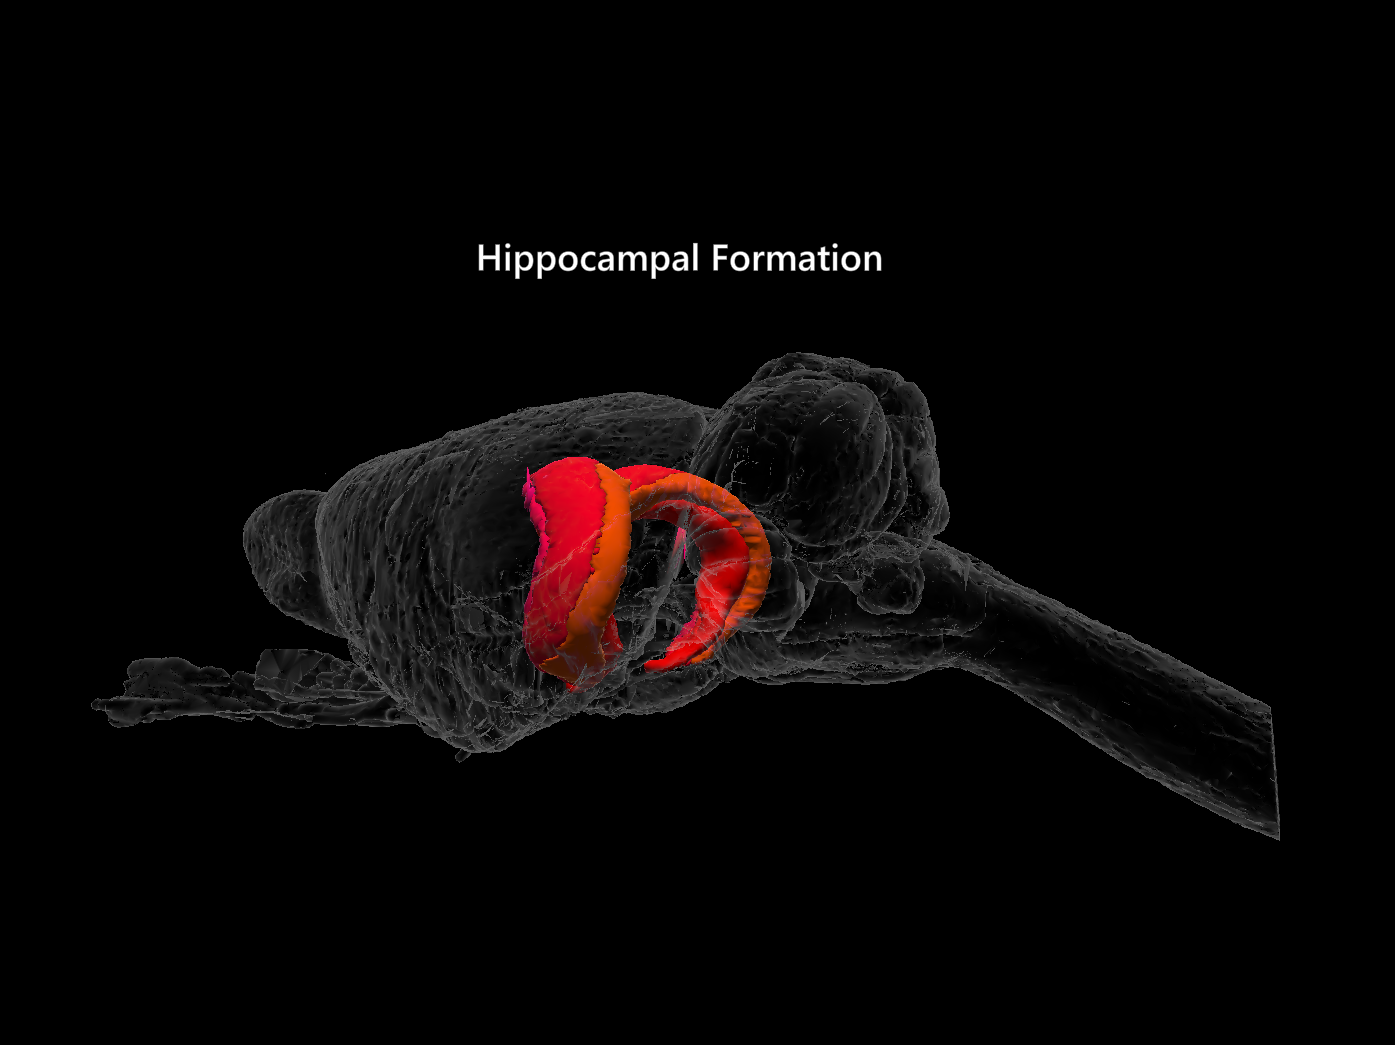
\includegraphics[width=0.33\textwidth]{fig/cluster2.png}
    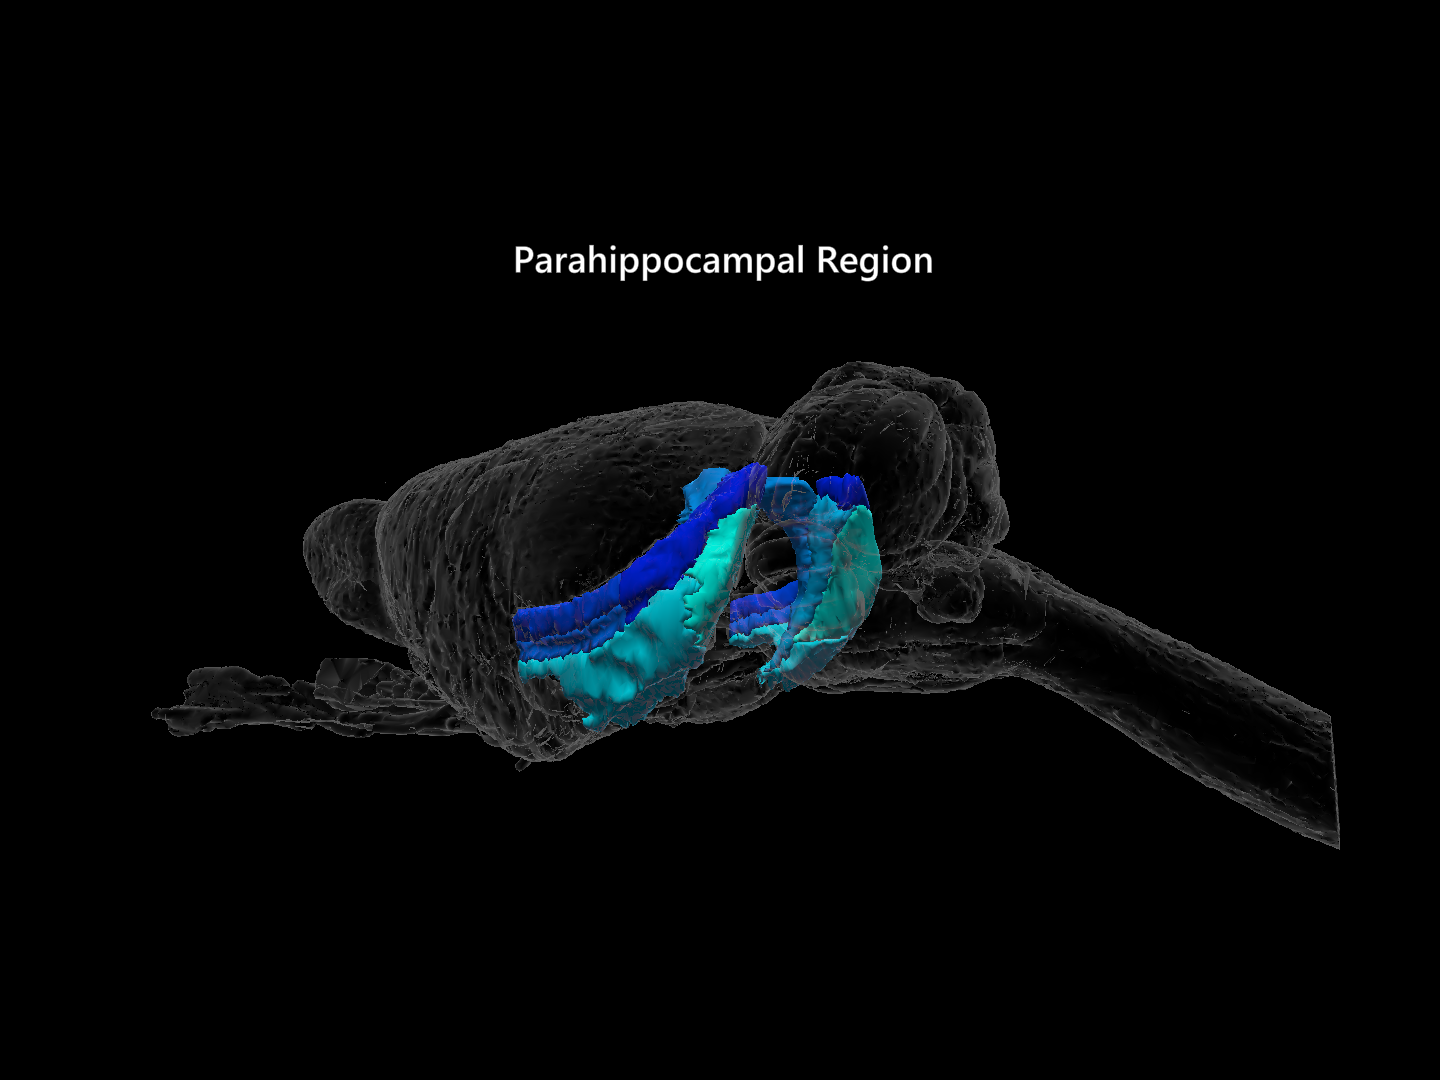
\includegraphics[width=0.33\textwidth]{fig/cluster3.png}
    \caption{Clusters in Nevrolens.}
    \label{fig:clustering}
\end{figure}


\subsection{Porting to Android}
% The application was originally developed for HoloLens 2, but other platforms were always in mind and because of the use of \nameref{chap:mrtk}, deploying to other platform was relatively easy, within the documentation for MRTK, there was guides for how to build for Android. Interaction on Android is more complicated though. Because all interaction happens on screen additional effort has to be laid down to implement a good user experience on smartphone.  

As MRTK is a framework specifically designed for HoloLens development, the HoloLens 2 naturally became the main focus of development and thus the application running on Android is a porting of the HoloLens version with small changes to somewhat accommodate the smartphone interface. It has however seen too little platform specific development and is in reality an incomplete product. It is however very much usable and can be seen as a great demonstration of the multiplatform capabilities of MRTK. 
Porting to Android was initially done by simply deploy the same application to Android, this is easily done in Unity with some MRTK tweaks which can be read up on in the \href{https://microsoft.github.io/MixedRealityToolkit-Unity/version/releases/2.2.0/Documentation/CrossPlatform/UsingARFoundation.html}{documentation}. While this works, some expected features are missing. For example, on the HoloLens 2 the user enables actions in a menu which is bound to their hand this is not possible in Android because the user interacts with the application not by moving the hand in space, but by touching the devices screen, therefore the application will simply disable the hand following feature on Android such that the menu buttons are static in space at all time. This is far from a optimal solution, but has worked for basic proof of concept. 
\begin{lstlisting}[language=c, caption={Basic example of separate features per device.}, label={item:androidcode}]
if (runtimePlatform != GlobalSettings.SupportedPlatform.HoloLens2)
{
    GetComponent<HandConstraintPalmUp>().enabled = false;
}
\end{lstlisting}

% There are of course some 


\subsection{Volumetric dissection plane}\label{chap:dissect}
\begin{figure}[ht]
    \centering
    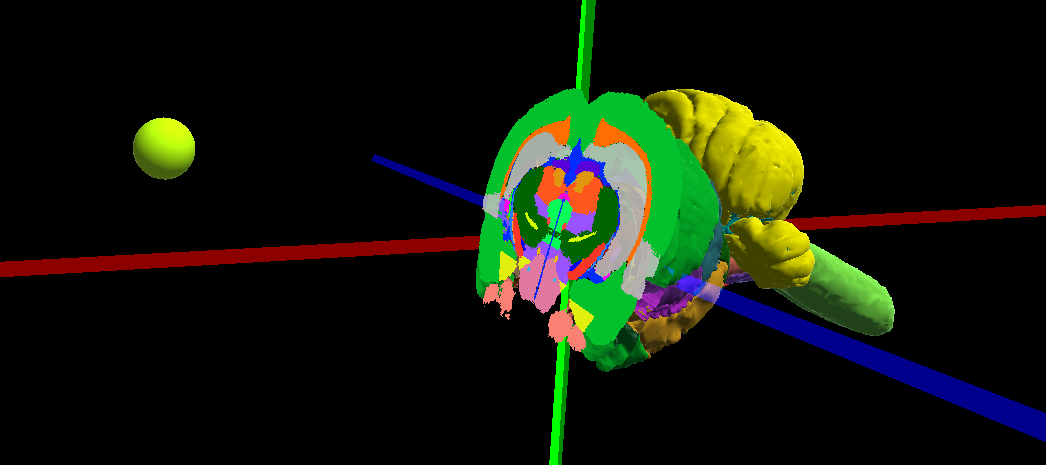
\includegraphics[width=0.7\textwidth]{fig/volumdissectionoverview.png}
    \caption{Volume dissection in Nevrolens}
\end{figure}

The basic implementation of clipping used for the dissection functionality leaves much to be desired. Clipping is a basic feature in most graphical libraries and shader languages, is will simply discard vertices which does not meet some set predicate. Its foremost purpose in computer graphics is to ensure that vertices outside the viewing cone will not be rendered, this to optimize render time. The result of this process on the surface model being cut open, such that the clipped part of the model becomes a empty hole to the inside of the model, this is illustrated on the left image of \autoref{fig:onoffvolume}. This can be solved by rasterizing the cut plane, and this was experimented with in this project with some success, however this functionality is not afforded by MRTKs standard shader, and thus implementation required the use of a custom shader, which meant that many other useful features implemented in the standard shader also had to be reimplemented. This lead to abandoning the solution and focusing instead on overlaying volumetric data upon the plane of dissection. 
\begin{figure}[ht]
    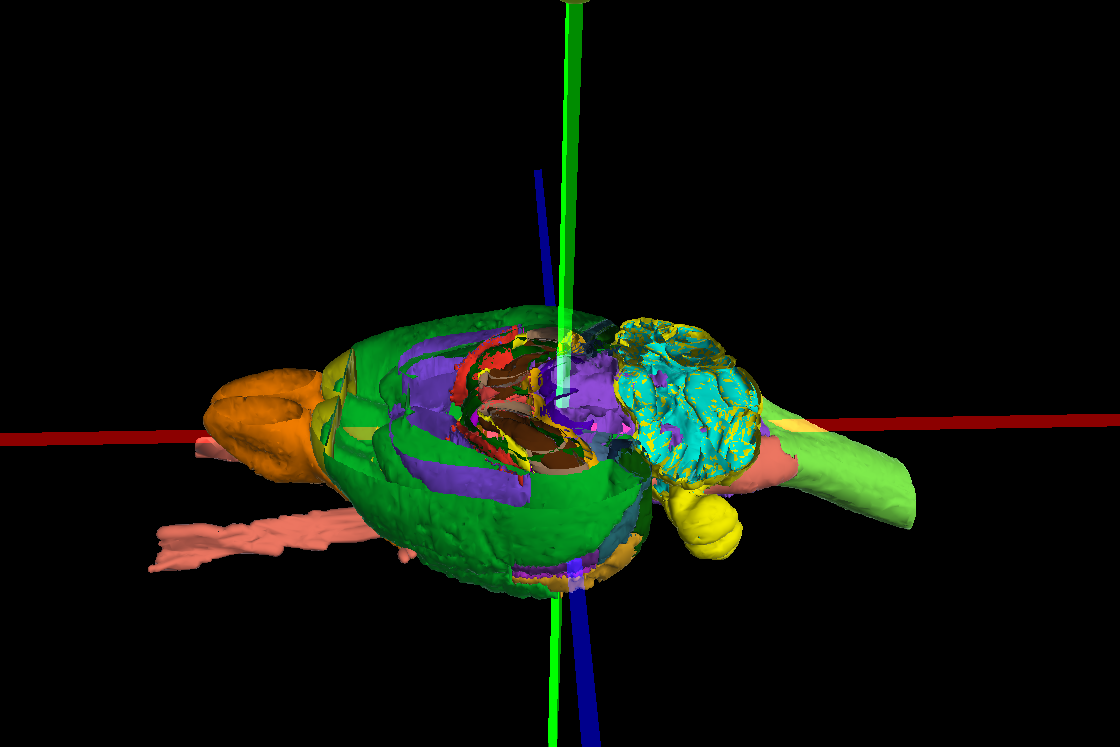
\includegraphics[width=0.5\textwidth , trim={3cm 2cm 4cm 5cm}, clip]{fig/top_mrtkdissect2.png}
    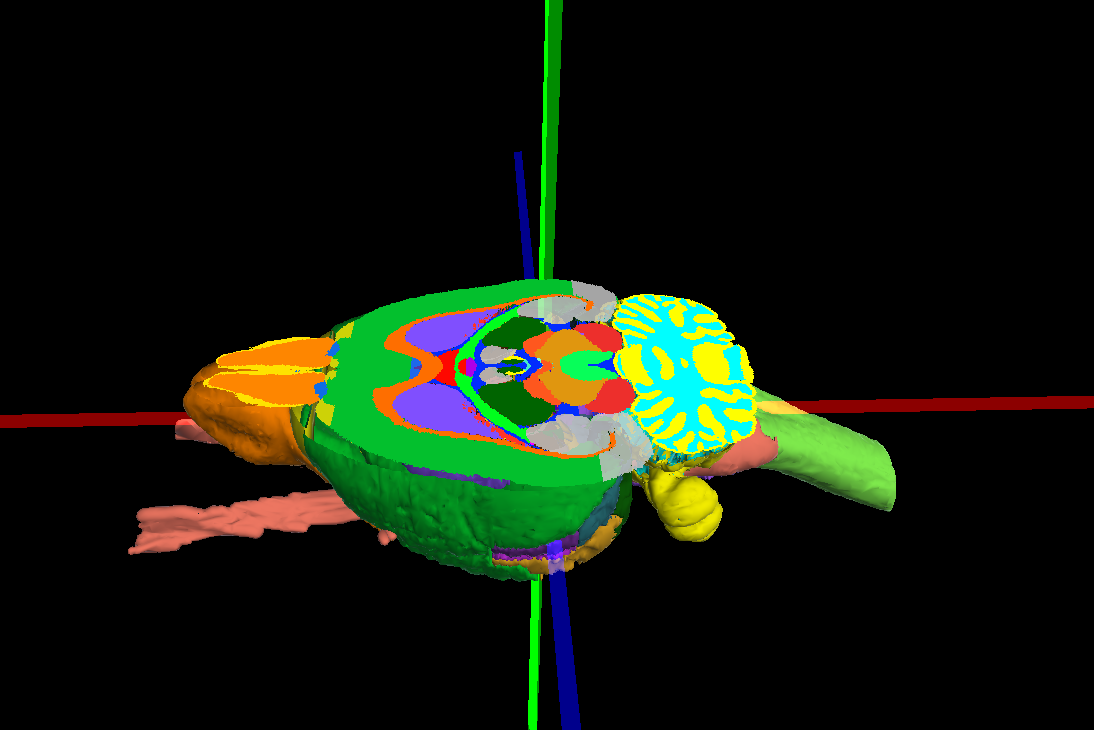
\includegraphics[width=0.5\textwidth , trim={3cm 2cm 4cm 5cm}, clip]{fig/top_volumedissect2.png}
    \caption{Dissection without and with volume plane.}
    \label{fig:onoffvolume}
\end{figure}
The Waxholm Space rat brain model is a volumetric data set, thus the goal with this feature was to visualize this data set as slices of the volume. The first step in this process was to format the volume in a manner that is usable in Unity and runnable on the target devices. The format of the WHS data set is the NIFTI format, this is a standardized format for neuroimaging data. With help from the library \href{https://github.com/plwp/Nifti.NET}{Nifti.NET} accessing the \texttt{ushort[]} 3d data array was made possible. An issue arising was that Unity struggled with parsing the data set, and this would result in the application freezing and no data array, thus a basic \textit{dotnet} console application called \href{https://github.com/ovravna/NevrolensNiftiTool}{NevrolensNiftiTool} was made to parse the NIFTI-file and output the 3d array as, of all things, a JSON object. JSON was chosen, after experimenting with \texttt{BinarySerialization}, but finding it to complex to use for data transfer, JSON was tested with success. The Unity scene \texttt{TextureBuilderScene} has a single purpose to generate a \texttt{Texture3D} resource from a JSON file. The MonoBehavior \texttt{BuildNifti3DTexture} takes the JSON file as input and outputs the data as a \texttt{Texture3D} Unity asset. This texture asset can than be used in later stages independent of the JSON file. 
With the data in the right format the first naïve implementation was using a MonoBehavior to apply a slice of the 3D data onto the \texttt{Texture2D} of a plane-object. This gave the desired effect of displaying a fixed slice of the volume, and by setting a free variable to one axis a sliding effect was made, however it was with the price of atrocious performance. For a robust implementation the feature would have to be excecated on the GPU as a shader. 

For the intended behavior, it was critical not just to generate slices along predefined axes, but to generate slices along arbitrary planes in the volume. This is, in theory, quite easy to implement on the shader by making use \textit{transformation matrices}. The idea is to map the UV coordinates of the default 2D texture onto the 3D volume. A basic implementation of this in the fragment shader can look like this:
\begin{lstlisting}[language=c]
fixed4 frag (v2f i) {
    // point from the 2D UV and the uniform float VariableSlider
    float3 uvw = float3(i.uv, VariableSlider);
    // tex3D samples the 3D texture NiftiTexture3D at point uvw
    fixed4 color = tex3D(NiftiTexture3D, uvw);
    return color;
}
\end{lstlisting}

This implementation will, just as the C\# MonoBehavior, display slices along the Z-axis. However, by simply multiplying the UV coordinate with a \texttt{TransformationMatrix} instead of setting the Z-coordinate, the result is the implementation of the shader used in this application. This one change makes the whole mapping process dependent on the TransformationMatrix, which makes the path forward very flexible.

\begin{lstlisting}[language=c]
fixed4 frag (v2f i) {
    // point cast from product of TransformMatrix and UV as 4d point
    float3 uvw = mul(TransformationMatrix, float4(i.uv, 0, 1));
    // tex3D samples the 3D texture NiftiTexture3D at point uvw
    fixed4 color = tex3D(NiftiTexture3D, uvw);
    return color;
}
\end{lstlisting}
\begin{figure}[ht]
    \centering
    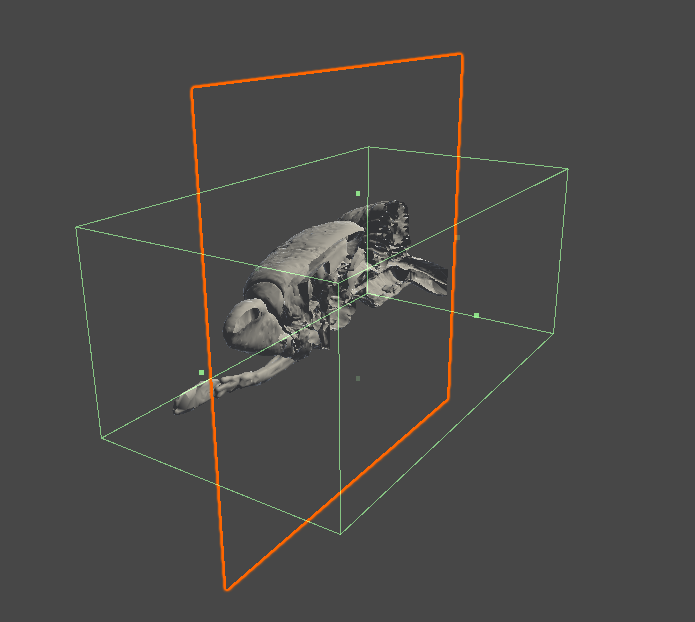
\includegraphics[width=0.5\textwidth]{fig/dissection_boxplaneview.png}
    % 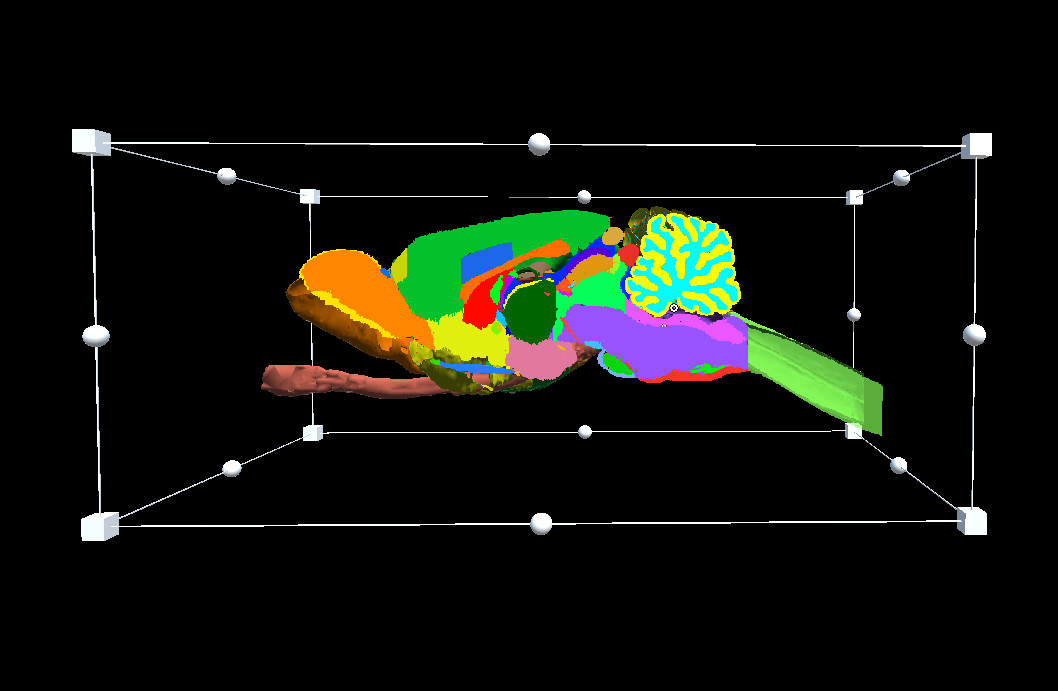
\includegraphics[width=0.4\textwidth]{fig/dissection_boxplanegame.png}
    \caption{The orange dissection plane and the green 1x2x1 cuboid brain model space.}
    \label{fig:boxandplanedissect}
\end{figure}

The affine transformations with matrices has built in support in Unity with the methods\\ \texttt{Matrix4x4.Translate(Vector3)}, \texttt{Matrix4x4.Rotate(Quaternion)}, \texttt{Matrix4x4.Scale(Vector3)} and a short hand for the product of all of these the \texttt{Matrix4x4.TRS(Vector3, Quaternion, Vector3)}. 
With the described implementation of the shader the aim will be to set the transformation matrix corresponding with a transformation from the clipping plane surface to a slice in the volumetric texture of the brain model, for arbitrary positions of the clipping plane relative to the brain model. This will be done by transforming through several vector spaces. As is custom with matrix multiplication these transformations will be explained in reverse order. 

% they will be described in the following 

The \texttt{tex3D} texture sampler on the shader samples textures as a 1x1x1 cube, with its center in (0.5, 0.5, 0.5), thus the output of the matrix transformation script must reflect this by mapping the UV coordinates to this space, lets call this the \textit{sampler space}. 

The model space of the geometric brain model has its center at the local origin and is a 1x2x1 cuboid. This \textit{brain model space} is illustrated as the green box in \autoref{fig:boxandplanedissect}. Additionally the geometric model is 180 degrees rotated on the X-axis relatively to the volumetric data, this is probably a result of swapped axis when creating either the volumetric data or the geometric data. Thus, the matrix transformation from brain model space to sampler space can look like this:

\begin{lstlisting}[language=c++]
Matrix4x4 modelToSamplerMatrix = Matrix4x4.TRS(
    new Vector3(0.5f, 0.5f, 0.5f),// translate center from origin
    Quaternion.Euler(180, 0, 0),  // rotational difference in models
    new Vector3(1, 0.5f, 1)       // scale down from 1x2x1 to 1x1x1
);
\end{lstlisting}

Transforming further from brain model space to the dissection plane space, colored orange in \autoref{fig:boxandplanedissect}, is done in to steps; from brain model to game world and from game world to dissection plane space. The matrices also, as oppose to the previous matrix, has to be calculated in the \texttt{Update} loop as it changes when the brain model or dissection plane is manipulated. These matrices are both trivial to implement as they use \texttt{Matrix4x4.TRS} with the \texttt{position}, \texttt{rotation} and \texttt{lossyScale} from each models \texttt{Transform} component.  This generates a model to world matrix, therefore the brain model matrix has to be Inversed. Lastly, a transformation is needed to offset the center of the dissection plane from the graphical origin in the upper left to the geometric origin in the center, this \texttt{planeOffsetMatrix} is a constant translation of (0.5, 0.5, 0). The final implementation will look like this:
% Unity provides the fields \texttt{Renderer.worldToLocalMatrix} and \texttt{Renderer.localToWorldMatrix} for this type of purpose, however the
\begin{lstlisting}[language=c++]
void Update() {
    worldToModelMatrix = Matrix4x4.TRS(
        model.position, model.rotation, model.lossyScale);

    worldToPlaneMatrix = Matrix4x4.TRS(
        plane.position, plane.rotation, plane.lossyScale);

    Matrix4x4 transformation = modelToSamplerMatrix 
                * Matrix4x4.Inverse(worldToModelMatrix)
                * worldToPlaneMatrix
                * planeOffsetMatrix;

    // moves the matrix to the shader as TransformationMatrix
    renderer.SetMatrix("TransformationMatrix", transformation);
}
\end{lstlisting}
The resulting plane will however be in grayscale as the \texttt{Texture3D} contains single \texttt{ushort} values per voxel, how this was fixed will be explored in \nameref{chap:braincolor}.

A last note is that there is a small, jet very noticeable, discrepancy between the volume model and the geometric model such that they do not completely overlap, \autoref{fig:onoffvolume} shows this to some extent. The researcher attributes this to the fact that different versions of the Waxholm Space brain are used in the generation of each volume and the lack of control in how the geometric model was created. Thus, when a single new data set is used for both geometric and volumetric models this issue should disappear.

\subsection{Coloring the brain}\label{chap:braincolor}

Throughout this thesis the reader will see the brain visualized in a number of different colors. Many images seen are of completely gray brains this are not and have never been part of the application, and are just for demonstration, this is how the model is seen in the Unity editor because color is set at runtime. The first iteration of coloring the brain structures, described in \autoref{chap:itr1}, was to use random colors. The goal of this was simply to visually distinguish the separate brain structures. An improvement was added which biased the random generation such that it generated lighter more saturated colors, but otherwise this was the state of brain colors until networking was implemented. With multiple users randomized colors was not appropriate anymore, because users would not be able to describe structures in terms of their color (unless the master client generates colors and distributes them to all, this approach was not taken). The properties needed from the colors was to be visually distinct and to be deterministically generated. This was implemented by sampling colors with uniform distance on the circumference of a circle of radius one inside the RGB-cube, like this. 
\begin{lstlisting}[caption={With \texttt{v} ranging from 0 to 2$\pi$.}]
float r = (Mathf.Sin(v) + 1) / 2;
float g = (Mathf.Cos(v) + 1) / 2;
float b = (-Mathf.Sin(v) + 1) / 2;
\end{lstlisting}
After some time the developer realized that smarter people than him already had solved this issue, and that the exact color properties needed was found in the HSV color model. The \textit{hue} channel in the HSV color model operates in the same manner as the code above when the other channels are constant. Thus by setting \textit{saturation} and \textit{value} to their max value and setting hue to the \texttt{v} from above mapped between zero and one, the resulting colors were basically the same only more saturated\footnote{The RGB implementation had a radius of 1, while $\sqrt{3}$ would (probably) give max saturation.}. The difference can be seen in \autoref{fig:hsvcolors}.

\begin{figure}[h]
    % 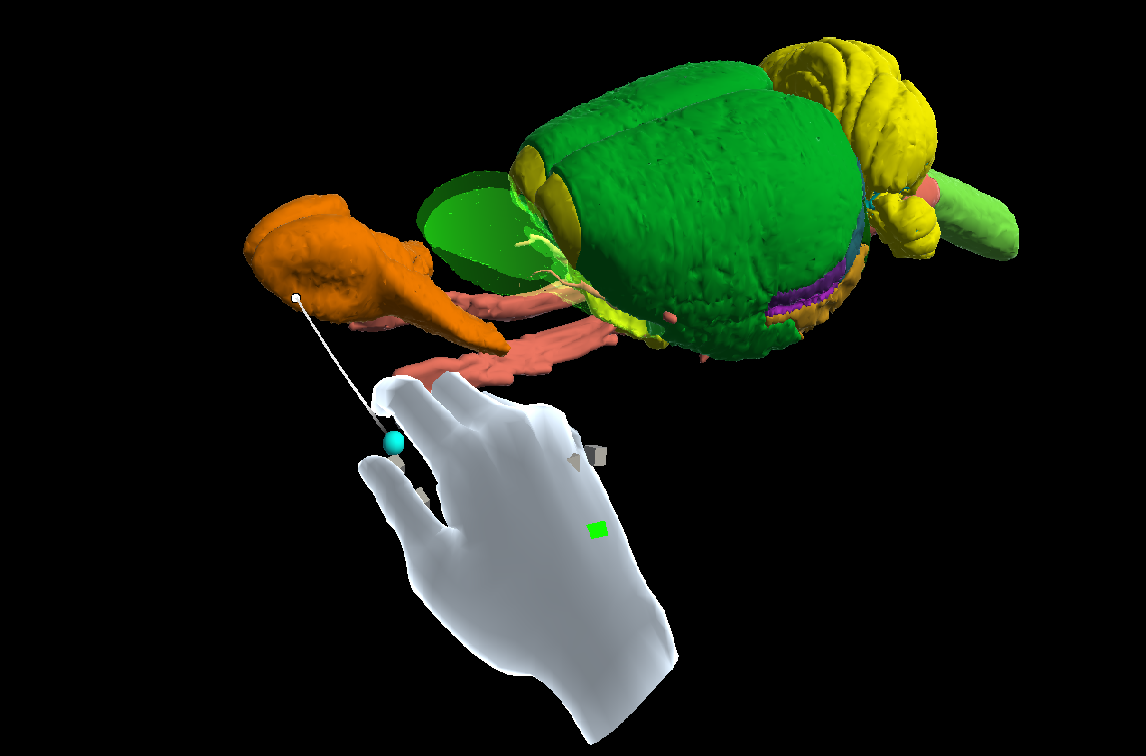
\includegraphics[width=0.65\textwidth]{fig/snaphint.png}
\centering
\begin{subfigure}[b]{0.4\textwidth}
    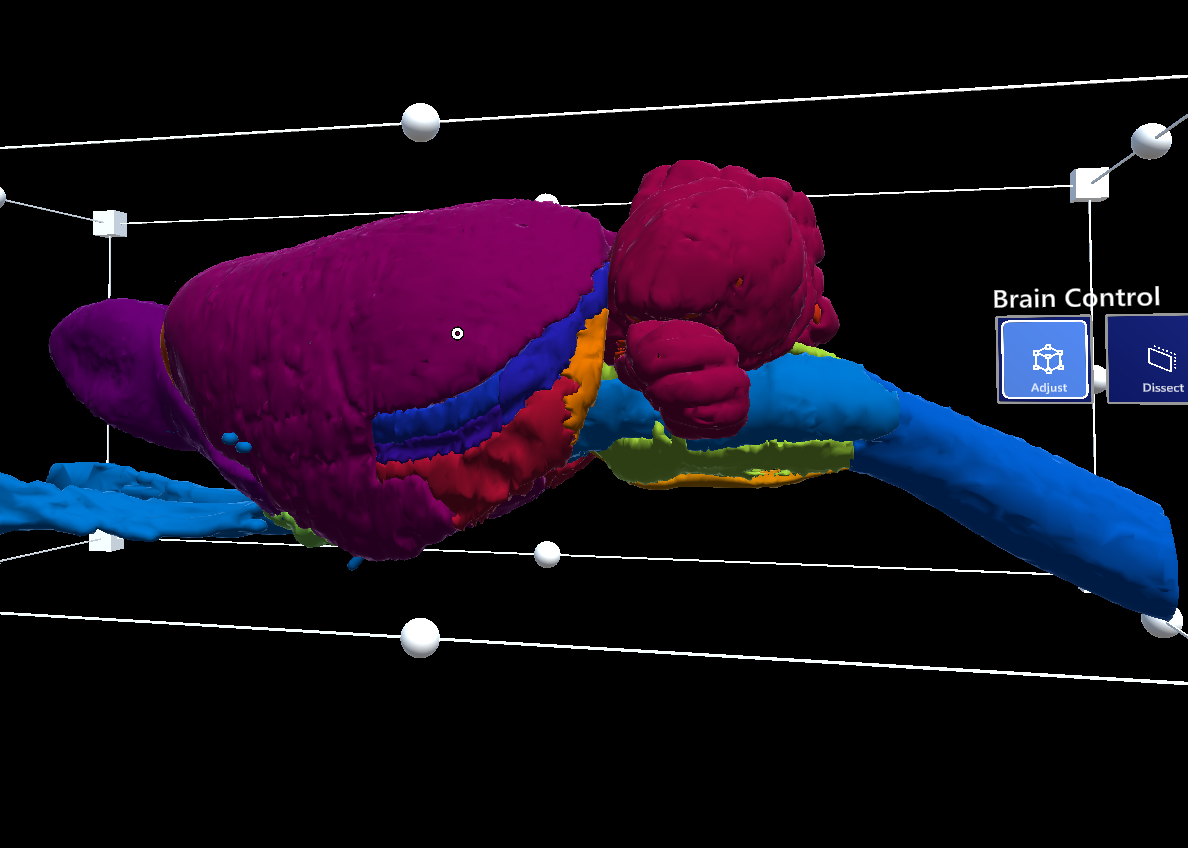
\includegraphics[width=\textwidth]{fig/nevrolens_brain_rgb_original.png}
    \caption{RGB implementation}
\end{subfigure}
\begin{subfigure}[b]{0.4\textwidth}
    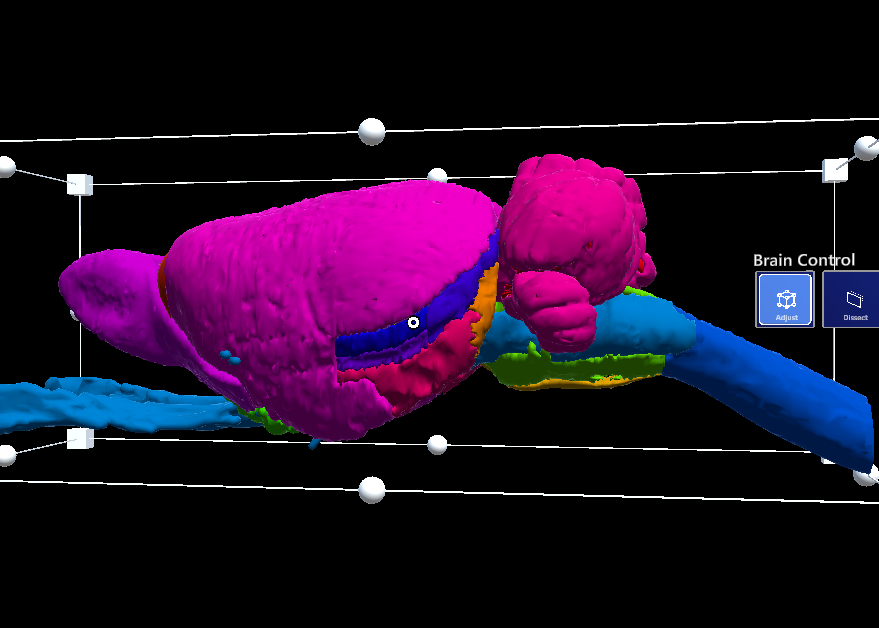
\includegraphics[width=\textwidth]{fig/nevrolens_brain_hsv_imitate.png}
    \caption{HSV implementation}
\end{subfigure}
\caption{}
\label{fig:hsvcolors}
\end{figure}

After demonstrating the application to neurologists, the developer was made aware that the Waxholm Space model has a predefined color model, and thus all the hard work was for naught. The final implementation consists of a parser of the LABLE-files in the Waxholm Space data set which contains color data. Then matching the name of the brain structure to its label and applying this color. The resulting colors can be seen in \autoref{chap:dissect}, e.g. in \autoref{fig:onoffvolume}. 
Though the HSV implementation is not used anymore for the brain coloring, the properties of this color model was found useful for other part of the application and is used to generate distinct colors for each user when in multiplayer and in clustering as seen in \autoref{fig:clustering}.

\subsubsection*{Coloring the dissection plane}
To color the dissect plane appropriate the same label colors as above as used, however the coloring of the structures in the plane happens on the shader so the color data had to be moved to the GPU. A 1D texture was used as a lookup table for the shader. The values in the volume \texttt{Texture3D} explored in \autoref{chap:dissect} are identifiers for the segmentation or brain structure the voxel is part of. These identifiers are defined in the label file, and thus by setting colors at the index of the identifier in the lookup table, the correct color could be sampled with \texttt{tex1D} in the shader.

\begin{lstlisting}
lookupTableLength = Labels.Last().identifier;
// Unity doesn't support 1D texture so it's 2D with height=1 
lookupTable = new Texture2D(width: lookupTableLength, height: 1);
foreach (var label : Labels)
    lookupTable.SetPixel(x: label.identifier, y: 0, label.color);

// moves the values to shader
renderer.SetFloat("LookupTableLength", lookupTableLength);
renderer.SetTexture("LookupTable", lookupTable);
\end{lstlisting}

The code above shows how the lookup table can be implemented. The fragment shader explored in \autoref{chap:dissect} can now be extended to sample these colors:
\begin{lstlisting}
fixed4 frag (v2f i) {
    float3 uvw = mul(TransformationMatrix, float4(i.uv, 0, 1));
    fixed4 voxel = tex3D(NiftiTexture3D, uvw);

    // maps 0 - 1 alpha channel, to 8-bit numbers
    float identifier = voxel.a * 256; 
    fixed4 color = tex1D(LookupTable, identifier / LookupTableLength)
    return color;
}
\end{lstlisting}

The volume texture is of the format \texttt{Alpha8} instead of the default \texttt{RGBA32}, this means that all its data is in the alpha channel and has a bit depth of eight, this could be done because all the data in the volume is the range 0 to 115, the range of identifiers in the label file. Thus, line 6 in the shader code above uses only the alpha value. 

% The texture is set to the format \texttt{Alpha8} such that each voxel is 8 bits instead of the 16 bits in the \texttt{ushort[]}, this is because the date only ranges from 0 to 115, 
% output for the matrix multiplication

% This will be done by transform through several spaces, \texttt{tex3D} space to brain model space 



% \autoref{chap:transformation} delves into detail on this topic. 






% \texttt{Quad}



% \footnote{Quads, like planes, are 2D surfaces in 3D space, but Quads are designed }



% this meant to create a \texttt{Texture3D} out


% Volumetric data of the Waxholm Space rat brain is a part of the open access data set, in fact the 




% Rotation in multiplayer space and such





\subsubsection*{}



% \subsection*{3rd iteration: Implementing network}
\subsection[Final Iteration]{Final Iteration}\label{chap:finaliter}






\subsubsection*{Networking optimization}



